\documentclass[preprint]{sigplanconf}

\usepackage{microtype}
\usepackage{textcomp}
\usepackage[scaled=0.9]{DejaVuSansMono}

\usepackage{balance}
\usepackage{moresize}
\usepackage{csquotes}
\usepackage{upgreek}

\usepackage{amsmath}
\usepackage{amssymb}
\usepackage{mathtools}
\usepackage{stmaryrd}

\usepackage{mathpartir}
\usepackage{galois}

\newtheorem{lemma}{Lemma}
\newtheorem{theorem}{Theorem}
\newtheorem{proposition}{Proposition}

\usepackage[usenames,dvipsnames]{color}
%\definecolor{PaleBlue}{rgb}{0.90,0.90,1.0}
%\definecolor{LightGray}{rgb}{0.90,0.90,0.90}
%\definecolor{CommentColor}{rgb}{0.76,0.45,0.12}
%\definecolor{OutputColor}{rgb}{0.59,0.00,0.59}

\definecolor{IdentifierColor}{rgb}{0.15,0.15,0.50}
\newcommand{\ID}[1]{{\color{IdentifierColor}#1}}

\definecolor{PuncColor}{rgb}{0.52,0.24,0.14}
\newcommand{\PN}[1]{{\color{PuncColor}#1}}

\definecolor{KeywordColor}{rgb}{0.52,0.24,0.14}
\newcommand{\KY}[1]{{\color{KeywordColor}#1}}

\definecolor{ValueColor}{rgb}{0.13,0.55,0.13}
\newcommand{\VL}[1]{{\color{ValueColor}#1}}

\definecolor{ResultColor}{rgb}{0.10,0.10,0.79}
\newcommand{\RE}[1]{{\color{ResultColor}#1}}

\definecolor{ErrorColor}{rgb}{0.75,0.10,0.10}
\newcommand{\EO}[1]{{\color{ErrorColor}#1}}


\usepackage{listings}
\lstset%
  {language=Lisp
  ,upquote=true
  ,mathescape=true
  ,basicstyle=\ttfamily\color{PuncColor}
  ,alsoletter=+-*/?'\#0123456789^:
  ,identifierstyle=\color{IdentifierColor}
  ,keywords=
    {define,let,match,if
    ,do,define-monad,for/monad+
    ,\#lang
    ,\#:when
    }
  ,keywordstyle=\color{KeywordColor}
  ,emph=
    {return,bind
    ,zero?
    ,ask-env,local-env
    ,ext,find,alloc
    ,get-store,put-store,update-store
    ,tell
    ,get-dead,put-dead,update-dead
    ,fail,mplus
    ,get-,put-,update-
    ,ask-,local-
    ,get-path-cond,refine
    }
  ,emphstyle=\color{IdentifierColor}\emph
  ,literate=
    {‹λ›}{{{\KY{«\uplambda»}}}}1
    {‹δ›}{{{\ID{«\updelta»}}}}1
    {‹σ›}{{{\ID{«\upsigma»}}}}1
    {‹ς›}{{{\ID{«\upvarsigma»}}}}1
    {‹ρ›}{{{\ID{«\uprho»}}}}1
    {‹φ›}{{{\ID{«\upphi»}}}}1
    {‹θ›}{{{\ID{«\uptheta»}}}}1
    {‹Σ›}{{{\ssmall\ID{«Σ»}}}}1
    {‹∅›}{{{\ID{«∅»}}}}1
    {‹←›}{{{\scriptsize«←»}}}1
    {‹≔›}{{{\scriptsize«≔»}}}1
    {‹₀›}{{{\ID{«\,⸤⦑0⦒⸥»}}}}1
    {‹₁›}{{{\ID{«\,⸤⦑1⦒⸥»}}}}1
    {‹₂›}{{{\ID{«\,⸤⦑2⦒⸥»}}}}1
    {‹′›}{{{\ID{«\,′»}}}}1
    {‹¢›}{{{\ID{\$}}}}1
    {‹∈›}{{{\ID{«∈»}}}}1
    {‹×›}{{{\ssmall\ID{«×»}}}}1
    {‹⊥›}{{{\ssmall\ID{«⊥»}}}}1
    {‹¬›}{{{\ssmall\ID{«¬»}}}}1
    {`}{{{\`{}}}}1
    {get-‹¢›}{{{\ID{\emph{get-\$}}}}}5
    {put-‹¢›}{{{\ID{\emph{put-\$}}}}}5
    {update-‹¢›}{{{\ID{\emph{update-\$}}}}}8
    {=}{{{\ID{=}}}}1
  ,classoffset=1
  ,keywords=
    {'add1,'sub1,'+,'-,'*,'quotient,'failure,'N
    ,\#t,\#f,0,1,2,3,4,5,6,7,8,9
    }
  ,keywordstyle=\color{ValueColor}
  }
\lstdefinestyle{result}
  {basicstyle=\ttfamily\color{ResultColor}
  ,keywordstyle=\color{ResultColor}
  ,identifierstyle=\color{ResultColor}
  ,literate=
    {‹λ›}{{{«\uplambda»}}}1
    {‹δ›}{{{«\updelta»}}}1
    {‹σ›}{{{«\upsigma»}}}1
    {‹ς›}{{{«\upvarsigma»}}}1
    {‹ρ›}{{{«\uprho»}}}1
    {‹φ›}{{{«\upphi»}}}1
    {‹θ›}{{{«\uptheta»}}}1
    {‹Σ›}{{{\ssmall«Σ»}}}1
    {‹∅›}{{{«∅»}}}1
    {‹←›}{{{«←»}}}1
    {‹≔›}{{{«≔»}}}1
    {‹₀›}{{{«\,⸤⦑0⦒⸥»}}}1
    {‹₁›}{{{«\,⸤⦑1⦒⸥»}}}1
    {‹₂›}{{{«\,⸤⦑2⦒⸥»}}}1
    {‹′›}{{{«\,′»}}}1
    {‹¢›}{{{\$}}}1
    {‹∈›}{{{«∈»}}}1
    {‹×›}{{{\ssmall«×»}}}1
    {‹⊥›}{{{\ssmall«⊥»}}}1
    {‹¬›}{{{\ssmall«¬»}}}1
    {timeout}{{{\EO{\emph{\textbf{timeout}}}}}}7
  }

\newcommand{\rfloat}[1]{\begin{flushright}\fbox{#1}\end{flushright}\vspace{-2.1em}}
\newcommand{\resultskip}{\vspace{-1.2em}}
\newcommand{\figskip}{\vspace{-1.3em}}
\newcommand{\up}[1]{\overbrace{\vphantom{X^X}#1}}

\begin{document}

% <<From Sigplan Template

\special{papersize=8.5in,11in}
\setlength{\pdfpageheight}{\paperheight}
\setlength{\pdfpagewidth}{\paperwidth}

%\conferenceinfo{CONF 'yy}{Month d--d, 20yy, City, ST, Country}
%\copyrightyear{20yy}
%\copyrightdata{978-1-nnnn-nnnn-n/yy/mm}
%\copyrightdoi{nnnnnnn.nnnnnnn}

%\titlebanner{banner above paper title}        % These are ignored unless
%\preprintfooter{short description of paper}   % 'preprint' option specified.

% >>

\title{Abstracting Definitional Interpreters}
%\subtitle{Subtitle Text, if any}

\authorinfo{}{}{}
%\authorinfo{David Darais}
%           {University of Maryland}
%           {darais@cs.umd.edu}
%\authorinfo{Nicholas Labich}
%           {University of Maryland}
%           {labichn@cs.umd.edu}
%\authorinfo{Phúc C. Nguyễn}
%           {University of Maryland}
%           {pcn@cs.umd.edu}
%\authorinfo{David Van Horn}
%           {University of Maryland}
%           {dvanhorn@cs.umd.edu}

\maketitle

\begin{abstract}
In this paper we show that definitional interpreters for programming languages
can express not only the usual notion of interpretation, but also a wide
variety of collecting semantics, abstract interpretations, symbolic executions
and their intermixings.
%
To achieve this we reconstruct a standard definitional interpreter using two
new ingredients: monadic operations and open recursion.
%
The resulting definitional \emph{abstract} interpreter is extensible and we
recover various abstract semantics through its instantiations.

In addition to recovering well-known abstractions, we show that the resulting
abstract interpreter is perfectly precise in modeling call and return flows,
\emph{i.e.} it implements Pushdown Control Flow Analysis (PDCFA).
%
True to the definitional style of Reynolds, the abstract interpreter contains
no explicit mechanics to achieve this property; it is simply inherited from the
defining metalanguage.

In addition to demonstrating our technique, we formalize a systematic
methodology for deriving definitional abstract interpreters, prove it sound,
and make precise its relationship to PDCFA.
\end{abstract}

%\category{CR-number}{subcategory}{third-level}
%\terms term1, term2
%\keywords keyword1, keyword2

\section{Introduction}

An abstract interpreter is intended to soundly and effectively compute
an over-approximation to its concrete counterpart.  For higher-order
languages, these concrete interpreters tend to be formulated as
state-machines~(e.g.~\cite{dvanhorn:jagannathan-weeks-popl95,
  dvanhorn:jagannathan-etal-popl98, 
  dvanhorn:wright-jagannathan-toplas98,
  dvanhorn:Might:2006:DeltaCFA,
  dvanhorn:midtgaard-jensen-sas-08,
  dvanhorn:Midtgaard2009Controlflow,
  dvanhorn:Might2011Family, dvanhorn:Sergey2013Monadic}).  There are
several reasons for this choice: they operate with simple transfer
functions defined over similarly simple data structures, they make
explicit all aspects of the state of a computation, and computing
fixed-points in the set of reachable states is straightforward.
%
The essence of the state-machine based approach was distilled by Van
Horn and Might in their ``abstracting abstract machines'' (AAM)
technique, which provides a systematic method for constructing
abstract interpreters from standard abstract machines like the CEK- or
Krivine-machines \cite{dvanhorn:VanHorn2010Abstracting}.  Language
designers who would like to build abstract interpreters and program
analysis tools for their language can now, in principle at least,
first build a state-machine interpreter and then turn the crank to
construct the approximating abstract counterpart.

A natural pair of questions that arise from this past work is to
wonder:
\begin{enumerate}
  \item can a systematic abstraction technique similar to AAM  be
carried out for interpreters written, \emph{not} as state-machines,
but instead as high-level definitional interpreters, i.e. recursive,
compositional evaluators?
\item  is such a perspective fruitful?
\end{enumerate}
In this functional pearl we seek to answer both questions in the
affirmative.

For the first question, we show the AAM recipe can be applied
to definitional interpreters in a straightforward adaptation of the
original method. The primary technical challenge in this new setting
is handling interpreter fixpoints in a way that is both sound and
always terminates---a naive abstraction of fixpoints will be sound but
isn't always terminating, and a naive use of caching for fixpoints
will guarantee termination but is inherently unsound. We address this
technical challenge with a straightforward caching fixpoint-finding
algorithm which is both sound guaranteed to terminate when abstracting
arbitrary definitional interpreters.

For the second question, we claim that the abstract definitional
interpreter perspective is fruitful in two regards.  The first is
unsurprising: high-level abstract interpreters offer the usual
beneficial properties of their concrete counterparts in terms of being
re-usable and extensible.  In particular, we show that abstract
interpreters can be structured with monad transformers to good effect.
The second regard is more surprising, and we consider its observation
to be the main contribution of this pearl.

Definitional interpreters, in contrast to abstract machines, can leave
aspects of computation implicit, relying on the semantics of the
defin\emph{ing}-language to define the semantics of the
defin\emph{ed}-language, an observation made by Reynolds in his landmark
paper, \emph{Definitional Interpreters for Higher-order Programming
  Languages}~\cite{dvanhorn:reynolds-acm72}.  For example, Reynolds showed it is
possible to write a definitional interpreter such that it defines a
call-by-value language when the metalanguage is call-by-value, and
defines a call-by-name language when the metalanguage is call-by-name.
Inspired by Reynolds, we show that \emph{abstract} definitional interpreters can likewise
inherit properties of the metalanguage.  In particular we construct an
abstract definitional interpreter where there is no explicit
representation of continuations or a call stack.  Instead the
interpreter is written in a straightforward recursive style, and the
call stack is implicitly handled by the metalangauge.  What emerges
from this construction is a total abstract evaluation function that
soundly approximates all possible concrete executions of a given
program.  But remarkably, since the abstract evaluator relies on the
metalanguage to manage the call stack implicitly, it is easy to
observe that it introduces no approximation in the matching of calls
and returns, and therefore implements a ``pushdown'' analysis, all
without the need for any explicit machinery to do so.

\subsection*{Outline}

In the remainder of this pearl, we present an adaptation of the AAM
method to the setting of recursively-defined, compositional evaluation
functions, a.k.a.~definitional interpreters.  We first briefly review
the basic ingredients in the AAM recipe (\S\ref{s:aam}) and then
define our definitional interpreter (\S\ref{s:interp}).  The
interpreter is largely standard, but is written in a monadic and
extensible style, so as to be re-usable for various forms of semantics
we examine.  The AAM technique applies in a basically straightforward
way by store-allocating bindings and soundly finitizing the heap.  But
when naively run, the interpreter will not always terminate.  To solve
this problem we introduce a caching strategy and a simple fixed-point
computation to ensure the interpreter terminates (\S\ref{s:cache}).
It is at this point that we observe the interpreter we have built
enjoys the ``pushdown'' property \emph{\`a la} Reynolds---it is
inherited from the defining language of our interpreter and requires
no explicit mechanism (\S\ref{s:reynolds}).

Having established the main results, we then explore some variations
in brief vignettes that showcase the flexibility of our definitional
abstract interpreter approach.  First we consider the widely used
technique of so-called ``store-widening,'' which trades precision for
efficiency by modelling the abstract store globally instead of locally
(\S\ref{s:widening}).  Thanks to our monadic formulation of the
interpreter, this is achieved by a simple re-ordering of the monad
transformer stack.  We also explore some alternative abstractions,
showing that due to the extensible construction, it's easy to
experiment with alternative components for the abstract interpreter.
In particular, we define an alternative interpretation of the primitive
operations that remains completely precise until forced by joins in
the store to introduce approximation (\S\ref{s:alt-abstraction}).  As
another variation, we explore computing a form of symbolic execution
as yet another instance of our interpreter (\S\ref{s:symbolic}).  Lastly, we
show how to incorporate so-called ``abstract garbage collection,'' a
well-known technique for improving the precision of abstract
interpretation by clearing out unreachable store locations, thus
avoiding future joins which cause imprecision (\S\ref{s:gc}).  This
last variation is significant because it demonstrates that even though
we have no explicit representation of the stack, it is possible to
compute analyses that typically require such explicit representations
in order to calculate root sets for garbage collection.

Finally, we place our work in the context of the prior literature on
higher-order abstract interpretation (\S\ref{s:related-work}) and draw
some conclusions (\S\ref{s:conclusion}).



%% In his landmark paper, \emph{Definitional Interpreters for Higher-order
%% Programming Languages}~\cite{dvanhorn:reynolds-acm72}, Reynolds observed that
%% when a programming language is defined by way of an interpreter, it is possible
%% to inherit semantic characteristics of the defining metalanguage. For example,
%% it is possible to define a definitional interpreter which is call-by-value when
%% the metalanguage is call-by-value, and call-by-name when the metalanguage is
%% call-by-name.

%% We expand on Reynolds's observation in the setting of abstract interpreters and
%% discover the following:
%% \begin{itemize}
%% \item Definitional interpreters, written in monadic style, can simultaneously
%%   define a language's semantics as well as safe approximations of those
%%   semantics, \emph{i.e.} abstract interpreters.
%% \item These definitional \emph{abstract} interpreters can inherit
%%   characteristics of the defining language.  In particular, precise
%%   call-and-return matching can be inherited, yielding a pushdown
%%   analysis~\cite{dvanhorn:Earl2010Pushdown,local:vardoulakis-diss12}.
%% \end{itemize}
%% Furthermore, we contribute:
%% \begin{itemize}
%% \item A systematic methodology for designing abstract interpreters via
%%   definitional interpreters; and
%% \item A soundness framework establishing the correctness of abstract
%%   interpreters defined in definitional style.
%% \end{itemize}

%% \paragraph{A Compositional Approach to Program Analysis}
%% There are many approaches to designing program analyzers for programming
%% languages. For \emph{higher-order} programming languages, two popular
%% approaches are to use abstract machines~\cite{dvanhorn:VanHorn2010Abstracting}
%% and constraint systems~\cite{dvanhorn:Neilson:1999}. Other foundations exist
%% for designing program analyzers, but no approach to-date utilizes big-step
%% operational semantics or definitional interpreters for program analysis of
%% higher-order languages. This is unfortunate because big-step semantics and
%% definitional interpreters are more compositional and high-level than state
%% machines or constraint systems. Big-step and denotational approaches exist for
%% first-order programming languages; the gap is in extending these ideas to the
%% higher-order setting.

%% We bridge this gap, providing the first framework for program analysis of
%% higher-order languages which builds upon big-step semantics and their
%% corresponding definitional interpreters, which are compositional by nature. 

%% Our key insights are to design definitional interpreters in monadic,
%% open-recursive style (§~\ref{s:interp}), and to design a
%% novel fixpoint algorithm tailored specifically to the setting of higher-order
%% definitional interpreters (§~\ref{s:cache}). The extensible nature of the
%% interpreter allows us to recover a wide-range of analyses through its
%% instantiation, including widening techniques (§~\ref{s:widening}), precision
%% preserving abstractions (§~\ref{s:alt-abstraction}), and symbolic execution for
%% program verification (§~\ref{s:symbolic}). Our implementation is freely
%% available through a suite of embedded languages in Racket (§~\ref{s:try-it}).
%% Finally, we prove the approach sound w.r.t. a derived big-step collecting and
%% abstract semantics (§~\ref{s:formalism}), where the key insight in the
%% formalism is to model not only standard big-step \emph{evaluation} relations,
%% but also big-step \emph{reachability} relations.

%% \paragraph{Pushdown Precision in Program Analysis}
%% A common problem with traditional approaches to control flow analysis is the
%% inability to properly match a function call with its return in the abstract
%% semantics. This leads to infeasible program (abstract) executions in which a
%% call is made from one point in the program, but control returns to another.
%% The PDCFA analysis of Earl \emph{et al}~\cite{dvanhorn:Earl2010Pushdown} and
%% CFA2 analysis of Vardoulakis and Shivers~\cite{dvanhorn:Vardoulakis2011CFA2}
%% were the first approaches to overcome this limitation in the higher-order
%% setting. In essence, these analyses replaces the traditional finite automata
%% abstractions of programs with pushdown automata, an approach pioneered by Reps
%% \emph{et al}~\cite{dvanhorn:Reps1995Precise} in the first-order setting.

%% We realize a new technique for defining abstract interpreters with pushdown
%% precision, meaning the analysis precisely matches function calls to returns. In
%% the setting of definitional interpreters, this property is inherited from the
%% defining metalanguage and requires no instrumentation to the analysis \emph{at
%% all} (§~\ref{s:reynolds}).

%% A technical difference between small-step and big-step approaches to semantics
%% are that small-step methods must model the execution context of evaluation,
%% whether through evaluation contexts~\cite{local:felleisen-TCS1992} or stack
%% frames~\cite{dvanhorn:Felleisen1987Calculus}. In big-step methods, there is no
%% model for the context; it is implicit in the definition of evaluation rules, or
%% in the case of definitional interpreters, implicit in the call-and-return
%% semantics of the defining programming language. Because a defining programming
%% language is precise in its call/return behavior, so is a definitional abstract
%% interpreter embedded within it.

\section{From Machines to Compositional Evaluators}
\label{s:aam}

In recent years, there has been considerable effort in the systematic
construction of abstract interpreters for higher-order languages using abstract
machines---first-order transition systems---as a semantic basis.  The so-called
\emph{Abstracting Abstract Machines} (AAM) approach to abstract
interpretation~\cite{dvanhorn:VanHorn2010Abstracting} is a recipe for
transforming a machine semantics into an easily abstractable form. The
transformation includes the following ingredients:
\begin{itemize}
\item Allocating continuations in the store;
\item Allocating variable bindings in the store;
\item Using a store that maps addresses to \emph{sets} of values;
\item Interpreting store updates as a join; and
\item Interpreting store dereference as a non-deterministic choice.
\end{itemize}
These transformations are semantics-preserving due to the original and derived
machines operating in a lock-step correspondence.  After transforming the
semantics in this way, a \emph{computable} abstract interpreter is achieved by:
\begin{itemize}
\item Bounding store allocation to a finite set of addresses; and
\item Widening base values to some abstract domain.
\end{itemize}
After performing these transformations, the soundness and computability of the
resulting abstract interpreter are then self-evident and easily proved.

The AAM approach has been applied to a wide variety of languages and
applications, and given the success of the approach it's natural to wonder what
is essential about its use of low-level machines. It is not at all clear
whether a similar approach is possible with a higher-level formulation of the
semantics, such as a compositional evaluation function defined recursively over
the syntax of expressions.

This paper shows that the essence of the AAM approach can be applied to a
high-level semantic basis.  We show that compositional evaluators written in
monadic style can express similar abstractions to that of AAM, and like AAM,
the design remains systematic.  Moreover, we show that the high-level semantics
offers a number of benefits not available to the machine model.  

\begin{figure} %{{{ f:syntax
\begin{mdframed}
\begin{alignat*}{4}
   e ∈ &&\mathrel{}   exp ⩴ &\mathrel{} 𝔥⸨(vbl⸩\ x𝔥⸨)⸩         &\hspace{3em} [⦑\emph{variable}⦒]
\\[\mathgobble]     &&\mathrel{}       ∣ &\mathrel{} 𝔥⸨(num⸩\ n𝔥⸨)⸩         &\hspace{3em} [⦑\emph{number}⦒]
\\[\mathgobble]     &&\mathrel{}       ∣ &\mathrel{} 𝔥⸨(lam⸩\ x\ e𝔥⸨)⸩      &\hspace{3em} [⦑\emph{lambda}⦒]
\\[\mathgobble]     &&\mathrel{}       ∣ &\mathrel{} 𝔥⸨(if0⸩\ e\ e\ e𝔥⸨)⸩   &\hspace{3em} [⦑\emph{conditional}⦒]
\\[\mathgobble]     &&\mathrel{}       ∣ &\mathrel{} 𝔥⸨(op2⸩\ b\ e\ e𝔥⸨)⸩   &\hspace{3em} [⦑\emph{binary op}⦒]
\\[\mathgobble]     &&\mathrel{}       ∣ &\mathrel{} 𝔥⸨(app⸩\ e\ e𝔥⸨)⸩      &\hspace{3em} [⦑\emph{application}⦒]
\\[\mathgobble]     &&\mathrel{}       ∣ &\mathrel{} 𝔥⸨(rec⸩\ x\ e\ e𝔥⸨)⸩   &\hspace{3em} [⦑\emph{letrec}⦒]
\\[\mathgobble] x ∈ &&\mathrel{}   var ≔ &\mathrel{} ❴𝔥⸨x⸩, 𝔥⸨y⸩, …❵        &\hspace{3em} [⦑\emph{variable names}⦒]
%\\[\mathgobble] u ∈ &&\mathrel{}  unop ≔ &\mathrel{} ❴𝔥⸨add1⸩, …❵           &\hspace{3em} [⦑\emph{unary prim}⦒]
\\[\mathgobble] b ∈ &&\mathrel{} binop ≔ &\mathrel{} ❴𝔥⸨+⸩, 𝔥⸨-⸩, …❵        &\hspace{3em} [⦑\emph{binary prim}⦒]
\end{alignat*}
\captionskip{Programming Language Syntax}
\label{f:syntax}
\end{mdframed}
\end{figure} %}}}

There is a rich body of work concerning tools and techniques for
\emph{extensible} interpreters~\cite{dvanhorn:Liang1995Monad,
  local:jaskelioff2009lifting, local:kiselyov2012typed}, all of which
applies to high-level semantics.  By putting abstract interpretation
for higher-order languages on a high-level semantic basis, we can
bring these results to bear on the construction of extensible abstract
interpreters.

\section{A Definitional Interpreter}\label{s:interp}

We begin by constructing a definitional interpreter for a small but
representative higher-order, functional language.  As our defining language, we
use an applicative subset of Racket, a dialect of Scheme.\footnote{This choice
is largely immaterial: any functional language would do.} The abstract syntax
of the language is defined in Figure~\ref{f:syntax}; it includes variables,
numbers, unary and binary operations on numbers, conditionals, {\tt letrec}
expressions, functions and applications.

\begin{figure} %{-{
\rfloat{⸨ev@⸩}
\begin{lstlisting}
¦ (define ((ev ev) e)
¦   (match e
¦     [(num n) (return n)]
¦     [(vbl x)
¦      (do ρ ← ask-env
¦          (find (ρ x)))]    
¦     [(ifz e₀ e₁ e₂) 
¦      (do v  ← (ev e₀)
¦          z? ← (zero? v)
¦          (ev (if z? e₁ e₂)))]
¦     [(op1 o e₀)
¦      (do v ← (ev e₀)
¦          (δ o v))]   
¦     [(op2 o e₀ e₁)
¦      (do v₀ ← (ev e₀)
¦          v₁ ← (ev e₁)
¦          (δ o v₀ v₁))]
¦     [(lrc f e₀ e₁) 
¦      (do ρ  ← ask-env
¦          a  ← (alloc f)
¦          ρ′ ≔ (ρ f a)
¦          (ext a (cons e₀ ρ′))
¦          (local-env ρ′
¦            (ev e₁)))]
¦     [(lam x e₀)
¦      (do ρ ← ask-env
¦          (return (cons (lam x e₀) ρ)))]
¦     [(app e₀ e₁)
¦      (do (cons (lam x e₂) ρ) ← (ev e₀)
¦          v₁ ← (ev e₁)
¦          a  ← (alloc x)         
¦          (ext a v₁)
¦          (local-env (ρ x a) 
¦            (ev e₂)))]))
\end{lstlisting}
\caption{The Extensible Definitional Interpreter}
\label{f:interpreter}
\end{figure} %}-}

The interpreter for the language is defined in Figure~\ref{f:interpreter}. At
first glance, it has many conventional aspects:
\begin{itemize}
\item It is compositionally defined by structural recursion on the syntax of
expressions.
\item It represents function values as a closure data structure which pairs the
function body with the evaluation environment.
\item It is structured monadically and uses monad operations to interact with
the environment and store.
\item It relies on a helper function ⸨δ⸩ to interpret primitive operations.
\end{itemize}
There are a few superficial aspects that deserve a quick note:
environments ⸨ρ⸩ are finite maps and ⸨(ρ«\ »x)⸩ denotes
«ρ(x)» while ⸨(ρ«\ »x a)⸩ denotes «ρ[x↦a]».  The
⸨do⸩-notation is just shorthand for ⸨bind⸩, as usual:

% LAYOUT
\begin{alignat*}{2}
   𝔥⸨(do x ←«\ »e . r)⸩ ≡ &\mathrel{} 𝔥⸨(bind e (λ«\ »(x) (do . r)))⸩
\\        𝔥⸨(do e . r)⸩ ≡ &\mathrel{} 𝔥⸨(bind e (λ«\ »(_) (do . r)))⸩
\\ 𝔥⸨(do x ≔«\ »e . r)⸩ ≡ &\mathrel{} 𝔥⸨(let ((x e)) (do . r))⸩
\\            𝔥⸨(do b)⸩ ≡ &\mathrel{} 𝔥⸨b⸩
\end{alignat*}
Finally, there are two unconventional aspects worth noting.

First, the interpreter is written in an \emph{open recursive style}; the
evaluator does not call itself recursively, instead it takes as an argument a
function ⸨ev⸩—shadowing the name of the function ⸨ev⸩ being defined—and ⸨ev⸩
(the argument) is called instead of self-recursion.  This is a standard
encoding for recursive functions in a setting without recursive binding.  It is
up to an external function, such as the Y-combinator, to close the recursive
loop.  This open recursive form is crucial for our purposes in that it allows
intercepting recursive calls to perform “deep” instrumentation of the
interpreter.

Second, the code is clearly \emph{incomplete}.  There are a number of free
variables, noted in italics, which must implement the following:
\begin{itemize}
\item The underlying monad of the interpreter: ⸨return⸩ and ⸨bind⸩;
\item An interpretation of primitives: ⸨δ⸩ and ⸨zero?⸩;
\item Environment operations: ⸨ask-env⸩ for retrieving the
environment and ⸨local-env⸩ for installing an environment;
\item Store operations: ⸨ext⸩ for updating the store, and ⸨find⸩ for
dereferencing locations; and
\item An operation for ⸨alloc⸩ating new store locations.
\end{itemize}
Going forward, we make frequent use of definitions involving free variables,
and we call such a collection of such definitions a \emph{component}. We assume
components can be named (in this case, we've named the component ⸨ev@⸩,
indicated by the box in the upper-right corner) and linked together to
eliminate free variables.\footnote{We use Racket
\emph{units}~\cite{local:flatt-pldi98} to model components in our
implementation.}

\begin{figure} %{-{
\rfloat{⸨monad@⸩}
\begin{alignat*}{1}
          & 𝔥⸨(define-monad⸩
\\[-0.5em]& ␣␣𝔥⸨(⸩\!\up{𝔥⸨ReaderT⸩}⸢env⸣\ 𝔥⸨(⸩\!\up{𝔥⸨FailT⸩}⸢errors⸣\ 𝔥⸨(⸩\!\up{𝔥⸨StateT⸩}⸢store⸣\ 𝔥⸨ID))))⸩
\end{alignat*}
\figskip\rfloat{⸨δ@⸩}
\begin{lstlisting}
¦ (define (δ . ovs)
¦   (match ovs
¦     [(list 'add1 n)  (return (add1 n))]
¦     [(list 'sub1 n)  (return (sub1 n))]
¦     [(list '- n)     (return (- n))]
¦     [(list '+ n₀ n₁) (return (+ n₀ n₁))]
¦     [(list '- n₀ n₁) (return (- n₀ n₁))]
¦     [(list '* n₀ n₁) (return (* n₀ n₁))]
¦     [(list 'quotient n₀ n₁)
¦      (if (= 0 n₁)
¦          fail
¦          (return (quotient n₀ n₁)))]))
¦ (define (zero? v)
¦   (return (= 0 v)))
\end{lstlisting}
\figskip\rfloat{⸨store@⸩}
\begin{lstlisting}
¦ (define (find a)
¦   (do σ ← get-store
¦       (return (σ a))))
¦ (define (ext a v) 
¦   (update-store (λ (σ) (σ a v))))
\end{lstlisting}
\figskip\rfloat{⸨alloc@⸩}
\begin{lstlisting}
¦ (define (alloc x)
¦   (do σ ← get-store
¦       (return (size σ))))
\end{lstlisting}
\caption{Components for Definitional Interpreters}
\label{f:concrete-components}
\end{figure} %}-}

\subsection{Instantiating the Interpreter}

Next we examine a set of components which complete the definitional
interpreter, defined in Figure~\ref{f:concrete-components}. The first component
is ⸨monad@⸩, which uses our ⸨define-monad⸩ macro to generate a set of bindings
based on a monad transformer stack.  For this interpreter, we use a failure
monad to model divide-by-zero errors, a state monad to model the store, and a
reader monad to model the environment.  The ⸨define-monad⸩ form generates
bindings for ⸨return⸩, ⸨bind⸩, ⸨ask-env⸩, ⸨local-env⸩, ⸨get-store⸩ and
⸨update-store⸩, and their definitions are
standard~\cite{dvanhorn:Liang1995Monad}. 

We also add the ⸨mrun⸩ operation for running monadic computations, starting
with the empty environment and store ⸨∅⸩:
\begin{lstlisting}
¦ (define (mrun m)
¦   (run-StateT ∅ (run-ReaderT ∅ m)))
\end{lstlisting}
While the ⸨define-monad⸩ form is hiding some details, this component could have
equivalently been written out explicitly. For example, ⸨return⸩ and ⸨bind⸩ can
be defined as:
\begin{lstlisting}
¦ (define (((return a) r) s) (cons a s))
¦ (define (((bind ma f) r) s)
¦   (match ((ma r) s)
¦     [(cons a s′) (((f a) r) s′)]
¦     ['failure 'failure]))
\end{lstlisting}
The remaining operations are similarly straightforward.  So far our use of
monad transformers can be seen as a mere convenience, but the monad abstraction
will become essential for deriving new analyses later on.

The ⸨δ@⸩ component defines the interpretation of primitives, which is given in
terms of the underlying monad.  Finally the ⸨alloc@⸩ component provides a
definition of ⸨alloc⸩, which fetches the store and uses its size to return a
fresh address (assuming the invariant «𝔥⸨(∈«\ »a σ)⸩ ⇔ 𝔥⸨a⸩ < 𝔥⸨(size σ)⸩»).
The ⸨store@⸩ component defines ⸨find⸩ and ⸨ext⸩ for finding and extending the
store in terms of the monadic operations.

The only remaing pieces of the puzzle are a fixed-point combinator, which is
straightforward to define:
\begin{lstlisting}
¦ (define ((fix f) x) ((f (fix f)) x))
\end{lstlisting}
and the main entry-point for the interpreter:
\begin{lstlisting}
¦ (define (eval e) (mrun ((fix ev) e)))
\end{lstlisting}
By taking advantage of Racket's languages-as-libraries
features~\cite{dvanhorn:TobinHochstadt2011Languages}, we construct REPLs for
interacting with this interpreter.  Here are a few examples, which make use of
a concrete syntax for more succinctly writing expressions. The identity
function evaluates to an answer consisting of a closure over the empty
environment together with the empty store:
ℑ⁅
¦ > (λ (x) x)
ℑ,
¦ '(((λ (x) x) . ()) . ())
ℑ⁆
Here's an example showing a non-empty environment and store:
ℑ⁅
¦ > ((λ (x) (λ (y) x)) 4)
ℑ,
¦ '(((λ (y) x) . ((x . 0))) . ((0 . 4)))
ℑ⁆
Primitive operations work as expected:
ℑ⁅
¦ > (* (+ 3 4) 9)
ℑ,
¦ '(63 . ())
ℑ⁆
And divide-by-zero errors result in failures:
ℑ⁅
¦ > (quotient 5 (- 3 3))
ℑ,
¦ '(failure . ())
ℑ⁆
Because our monad stack places ⸨FailT⸩ above ⸨StateT⸩, the answer includes the
(empty) store at the point of the error. Had we changed ⸨monad@⸩ to use:
\begin{alignat*}{1}
& ␣␣𝔥⸨(⸩\!\up{𝔥⸨ReaderT⸩}⸢env⸣\ 𝔥⸨(⸩\!\up{𝔥⸨StateT⸩}⸢store⸣\ 𝔥⸨(⸩\!\up{𝔥⸨FailT⸩}⸢errors⸣\ 𝔥⸨ID⸩))))
\end{alignat*}
failures would not include the store:
ℑ⁅
¦ > (quotient 5 (- 3 3))
ℑ,
¦ 'failure
ℑ⁆
At this point we've defined a simple definitional interpreter, although the
extensible components involved—monadic operations and open recursion—will allow
us to instantiate the same interpreter to achieve a wide range of useful
abstract interpretations.

\subsection{Collecting Variations}\label{s:collecting}

The formal development of abstract interpretation often starts from a so-called
``non-standard collecting semantics.''  A common form of collecting semantics
is a trace semantics, which collects streams of states the interpreter reaches.
Figure~\ref{f:trace} shows the monad stack for a tracing interpreter and a
``mix-in'' for the evaluator.  The monad stack adds ⸨WriterT⸩ using ⸨List⸩,
which provides a new operation ⸨tell⸩ for writing items to the stream of
reached states.  The ⸨ev-trace⸩ function is a wrapper around an underlying
⸨ev₀⸩ unfixed evaluator, and interposes itself between each recursive call by
⸨tell⸩ing the current state of the evaluator, that is the current expression,
environment, and store.  The top-level evaluation function is then:
\begin{lstlisting}
¦ (define (eval e) 
¦   (mrun ((fix (ev-tell ev)) e)))
\end{lstlisting}

\begin{figure} %{-{
\rfloat{⸨trace-monad@⸩}
\begin{alignat*}{1}
          & 𝔥⸨(define-monad⸩
\\[-0.5em]& ␣␣𝔥⸨(⸩\!\up{𝔥⸨ReaderT⸩}⸢env⸣\ 𝔥⸨(⸩\!\up{𝔥⸨FailT⸩}⸢errors⸣\ 𝔥⸨(⸩\!\up{𝔥⸨StateT⸩}⸢store⸣\ 𝔥⸨(⸩\!\up{𝔥⸨WriterT List⸩}⸢traces⸣\ 𝔥⸨ID)))))⸩
\end{alignat*}
\figskip\rfloat{⸨ev-tell@⸩}
\begin{lstlisting}
¦ (define (((ev-tell ev₀) ev) e)
¦   (do ρ ← ask-env
¦       σ ← get-store
¦       (tell (list e ρ σ))
¦       ((ev₀ ev) e)))
\end{lstlisting}
\caption{Trace Collecting Semantics}
\label{f:trace}
\end{figure} %}-}

Now when an expression is evaluated, we get the resulting answer and a list of
all the states seen by the evaluator, in the order in which they were seen. For
example:
ℑ⁅
¦ > (* (+ 3 4) 9)
ℑ,
¦ '((63 . ())
¦   ((* (+ 3 4) 9)()())
¦   ((+ 3 4) () ())
¦   (3 () ())
¦   (4 () ())
¦   (9 () ()))
ℑ⁆
% ℑ⁅
% ¦ > ((λ (x) (λ (y) x)) 4)
% ℑ,
% ¦ '((((λ (y) x) . ((x . 0))) . ((0 . 4)))
% ¦   (((λ (x) (λ (y) x)) 4) () ())
% ¦   ((λ (x) (λ (y) x)) () ())
% ¦   (4 () ())
% ¦   ((λ (y) x) ((x . 0)) ((0 . 4))))
% ℑ⁆
Were we to swap ⸨List⸩ with ⸨Set⸩ in the monad stack, we would obtain a
\emph{reachable} state semantics, another common form of collecting semantics,
that loses the order and repetition of states.

As another collecting semantics variant, we show how to collect the \emph{dead
code} in a program.  Here we use a monad stack that has an additional state
component (with operations named ⸨put-dead⸩ and ⸨get-dead⸩) which stores the
set of dead expressions.  Initially this will contain all of the subexpressions
of the program.  As the interpreter recurs through expressions it will remove
them from the dead set.

Figure~\ref{f:dead} defines the monad stack for the dead code collecting
semantics and the ⸨ev-dead@⸩ component, another mix-in for an ⸨ev₀⸩ evaluator
to remove the given subexpression before recurring.  Since computing the dead
code requires an outer wrapper that sets the initial set of dead code to be all
of the subexpressions in the program, we define ⸨eval-dead@⸩ which consumes a
\emph{closed evaluator}, i.e. something of the form ⸨(fix ev)⸩.

Putting these pieces together, the dead code collecting semantics is defined:
\begin{lstlisting}
¦ (define (eval e)
¦   (mrun ((eval-dead (fix (ev-dead ev))) e)))
\end{lstlisting}
Running a program with the dead code interpreter produces an answer and the set
of expressions that were not evaluated during the running of a program:
ℑ⁅
¦ > (if0 0 1 2)
ℑ,
¦ (cons '(1 . ()) (set 2))
ℑ;
¦ > (* (+ 3 4) 9)
ℑ,
¦ (cons '(63 . ()) (set))
ℑ;
¦ > (λ (x) x)
ℑ,
¦ (cons '(((λ (x) x) . ()) . ()) (set 'x))
ℑ;
¦ > (if0 (quotient 1 0) 2 3)]
ℑ,
¦ (cons '(failure . ()) (set 3 2))
ℑ⁆

\begin{figure} %{-{
\rfloat{⸨dead-monad@⸩}
\begin{alignat*}{1}
          & 𝔥⸨(define-monad⸩
\\[-0.5em]& ␣␣𝔥⸨(⸩\!\up{𝔥⸨ReaderT⸩}⸢env⸣\ 𝔥⸨(⸩\!\up{𝔥⸨StateT⸩}⸢store⸣\ 𝔥⸨(⸩\!\up{𝔥⸨StateT⸩}⸢dead⸣\ 𝔥⸨(⸩\!\up{𝔥⸨FailT⸩}⸢errors⸣\ 𝔥⸨ID)))))⸩
\end{alignat*}
\figskip\rfloat{⸨ev-dead@⸩}
\begin{lstlisting}
¦ (define (((ev-dead ev₀) ev) e)
¦   (do θ  ← get-dead       
¦       (put-dead (set-remove θ e))
¦       ((ev₀ ev) e)))
\end{lstlisting}
\figskip\rfloat{⸨eval-dead@⸩}
\begin{lstlisting}
¦ (define ((eval-dead eval) e₀)
¦   (do (put-dead (subexps e₀))
¦       (eval e₀)))
\end{lstlisting}
\caption{Dead Code Collecting Semantics}
\label{f:dead}
\end{figure} %}-}

Our setup makes it easy not only to express the concrete interpreter, but also
different forms of collecting semantics. Let us now look at abstractions.

\subsection{Abstracting Base Values}\label{s:base}

Our interpreter must become decidable before it can be considered an analysis,
and the first step towards decidability is to abstract the base types of the
language to something finite. We do this for our number base type by
introducing a new \emph{abstract} number, written ⸨'N⸩, which represents the
set of all numbers. Abstract numbers are introduced by an alternative
interpretation of primitive operations, given in Figure~\ref{f:abs-delta},
which simply produces ⸨'N⸩ in all cases. 

Some care must be taken in the abstract interpretation of ⸨'quotient⸩. If the
denominator is the abstract number ⸨'N⸩, then it is possible the program could
fail as a result of divide-by-zero, since ⸨0⸩ is contained in the
representation of ⸨'N⸩. Therefore there are \emph{two} possible answers when
the denominator is ⸨'N⸩: ⸨'N⸩ and ⸨'failure⸩. Both answers are ⸨return⸩ed by
introducing non-determinism ⸨NondetT⸩ into the monad stack:
\begin{alignat*}{1}
& 𝔥⸨(⸩\!\up{𝔥⸨ReaderT⸩}⸢env⸣\ 𝔥⸨(⸩\!\up{𝔥⸨FailT⸩}⸢errors⸣\ 𝔥⸨(⸩\!\up{𝔥⸨StateT⸩}⸢store⸣𝔥\ 𝔥⸨(⸩\!\up{𝔥⸨NondetT⸩}⸢branching⸣\ 𝔥⸨ID))))⸩
\end{alignat*}
Adding non-determinism provides the ⸨mplus⸩ operation for combining multiple
answers. Non-determinism is also used in the implementation of ⸨zero?⸩, which
returns both true and false on ⸨'N⸩.

\begin{figure} %{-{
\rfloat{⸨δ^@⸩}
\begin{lstlisting}
¦ (define (δ . ovs)
¦   (match ovs
¦     [(list 'add1 n)  (return 'N)]
¦     [(list 'sub1 n)  (return 'N)]
¦     [(list '+ n₀ n₁) (return 'N)]
¦     [(list '- n₀ n₁) (return 'N)]
¦     [(list '* n₀ n₁) (return 'N)]
¦     [(list 'quotient n₀ (? number? n₁))
¦      (if (= 0 n₁) fail (return 'N))]
¦     [(list 'quotient n₀ 'N)
¦      (mplus fail (return 'N))]))
¦ (define (zero? v)
¦   (match v
¦     ['N (mplus (return #t) (return #f))]
¦     [_  (return (= 0 v))]))
\end{lstlisting}
\caption{Abstracting Primitive Operations}
\label{f:abs-delta}
\end{figure} %}-}

By linking together ⸨δ^@⸩ and the monad stack with non-determinism, we obtain
an evaluator that produces a set of results:
ℑ⁅
¦ > (* (+ 3 4) 9)
ℑ,
¦ '((N . ()))
ℑ;
¦ > (quotient 5 (add1 2))
ℑ,
¦ '((failure . ()) (N . ()))
ℑ;
¦ > (if0 (add1 0) 3 4)
ℑ,
¦ '((3 . ()) (4 . ()))
ℑ⁆

If we link ⸨δ^@⸩ with the \emph{tracing} monad stack plus non-determinism:
\begin{alignat*}{1}
  & 𝔥⸨(⸩\!\up{𝔥⸨ReaderT⸩}⸢env⸣𝔥⸨(⸩\!\up{𝔥⸨FailT⸩}⸢errors⸣𝔥⸨(⸩\!\up{𝔥⸨StateT⸩}⸢store⸣
    𝔥⸨(⸩\!\up{𝔥⸨WriterT List⸩}⸢traces⸣𝔥⸨(⸩\!\up{𝔥⸨NondetT⸩}⸢branching⸣\ 𝔥⸨ID)⸩\!…\!𝔥⸨)⸩
\end{alignat*}
we get an evaluator that produces sets of traces:
ℑ⁅
¦ > (if0 (add1 0) 3 4)
ℑ,
¦ (set
¦  '((3 . ())
¦    ((if0 (add1 0) 3 4) () ())
¦    ((add1 0) () ())
¦    (0 () ())
¦    (3 () ()))
¦  '((4 . ())
¦    ((if0 (add1 0) 3 4) () ())
¦    ((add1 0) () ())
¦    (0 () ())
¦    (4 () ())))
ℑ⁆

It should be clear that the interpreter will only ever see a finite set of
numbers (including ⸨'N⸩), but it's definitely not true that the interpreter
halts on all inputs.  First, it's still possible to generate an infinite number
of closures.  Second, there's no way for the interpreter to detect when it sees
a loop.  To make a terminating abstract interpreter requires tackling both.  We
look next at abstracting closures.

\subsection{Abstracting Closures}

Closures consist of code---a lambda term---and an environment---a finite map
from variables to addresses.  Since the set of lambda terms and variables is
bounded by the program text, it suffices to abstract closures by abstracting
the set of addresses.  Following the AAM approach, we can do this by modifying
the allocation function to always produce elements drawn from a finite set.  In
order to retain soundness in the semantics, we will need to modify the store to
map addresses to \emph{sets} of values and model store update as a join and
dereference as a non-deterministic choice.

Any abstraction of the allocation function that produces a finite set will do,
but the choice of abstraction will determine the precision of the resulting
analysis.  A simple choice is to allocate variable bindings by using a
variable's name as its address.  This gives a monomorphic, or 0CFA-like,
abstraction.

Figure~\ref{f:0cfa-abs} shows an alternative component for finite
allocation that uses variables names as the notion of addresses and a
component for the derived operations ⸨find⸩ and ⸨ext⸩
when the store uses a \emph{set} as its range.  The
⸨for/monad+⸩ form is just a convenience for combining a set of
computations with ⸨mplus⸩; in other words, ⸨find⸩
returns \emph{all} of the values in the store at a given address.  The
⸨ext⸩ function joins whenever an address is already allocated,
otherwise it maps the address to a singleton set.

\begin{figure}
\rfloat{⸨alloc^@⸩}
\begin{lstlisting}
(define (alloc x)
  (return x))
\end{lstlisting}
\figskip\rfloat{⸨store-nd@⸩}
\begin{lstlisting}
¦ (define (find a)
¦   (do σ ← get-store
¦       (for/monad+ ([v (σ a)])
¦         (return v))))
¦ (define (ext a v)
¦   (update-store
¦     (λ (σ) (σ a (if (∈ a σ) 
¦                     (set-add (σ a) v) 
¦                     (set v))))))
\end{lstlisting}
\caption{Abstracting Allocation: 0CFA}
\label{f:0cfa-abs}
\end{figure}

By linking these components together with the same monad stack from
Section~\ref{s:base}, we obtain an interpreter that loses precision whenever
variables are bound to multiple values.  For example, this program
binds ⸨x⸩ to both ⸨0⸩ and ⸨1⸩ and therefore
produces both answers when run:
ℑ⁅
¦ > (let f (λ (x) x)
¦     (let _ (f 0) (f 1)))]
ℑ,
¦ '((0 . ((x 1 0) (f ((λ (x) x) . ()))))
¦   (1 . ((x 1 0) (f ((λ (x) x) . ())))))
ℑ⁆

We've now taken care of making a sound, finite abstraction of the
space of all closures that arise during evaluation.  It would seem we
are very close to having a sound, total abstract interpretation
function.


\section{Abstracting Closures}\label{s:closures}

Closures consist of code---a lambda term---and an environment---a finite map
from variables to addresses.  Since the set of lambda terms and variables is
bounded by the program text, it suffices to abstract closures by abstracting
the set of addresses.  Following the AAM approach, we can do this by modifying
the allocation function to always produce elements drawn from a finite set.  In
order to retain soundness in the semantics, we will need to modify the store to
map addresses to \emph{sets} of values and model store update as a join and
dereference as a non-deterministic choice.

Any abstraction of the allocation function that produces a finite set will do,
but the choice of abstraction will determine the precision of the resulting
analysis.  A simple choice is to allocate variable bindings by using a
variable's name as its address.  This gives a monomorphic, or 0CFA-like,
abstraction.

Figure~\ref{f:0cfa-abs} shows an alternative component for finite
allocation that uses variables names as the notion of addresses and a
component for the derived operations ⸨find⸩ and ⸨ext⸩
when the store uses a \emph{set} as its range.  The
⸨for/monad+⸩ form is just a convenience for combining a set of
computations with ⸨mplus⸩; in other words, ⸨find⸩
returns \emph{all} of the values in the store at a given address.  The
⸨ext⸩ function joins whenever an address is already allocated,
otherwise it maps the address to a singleton set.

\begin{figure}
\rfloat{⸨alloc^@⸩}
\begin{lstlisting}
(define (alloc x)
  (return x))
\end{lstlisting}
\figskip\rfloat{⸨store-nd@⸩}
\begin{lstlisting}
¦ (define (find a)
¦   (do σ ← get-store
¦       (for/monad+ ([v (σ a)])
¦         (return v))))
¦ (define (ext a v)
¦   (update-store
¦     (λ (σ) (σ a (if (∈ a σ) 
¦                     (set-add (σ a) v) 
¦                     (set v))))))
\end{lstlisting}
\caption{Abstracting Allocation: 0CFA}
\label{f:0cfa-abs}
\end{figure}

By linking these components together with the same monad stack from
Section~\ref{s:base}, we obtain an interpreter that loses precision whenever
variables are bound to multiple values.  For example, this program
binds ⸨x⸩ to both ⸨0⸩ and ⸨1⸩ and therefore
produces both answers when run:
ℑ⁅
¦ > (let f (λ (x) x)
¦     (let _ (f 0) (f 1)))]
ℑ,
¦ '((0 . ((x 1 0) (f ((λ (x) x) . ()))))
¦   (1 . ((x 1 0) (f ((λ (x) x) . ())))))
ℑ⁆

We've now taken care of making a sound, finite abstraction of the
space of all closures that arise during evaluation.  It would seem we
are very close to having a sound, total abstract interpretation
function.


\section{Detecting Cycles with a Cache}\label{s:cache}

At this point, it's worth observing that the interpreter obtained by
linking together ⸨δ^@⸩ and ⸨alloc^@⸩ components will
only ever visit a finite number of states for a given program.  The
state consists of an expression, environment, and store mapping
addresses to sets of values.  To see that this is a finite set is
pretty straightforward: expressions (in the given program) are finite,
environments are maps from variables (again, finite in a program) to
address.  The addresses are finite thanks to ⸨alloc^⸩, so
environments are finite.  The store maps addresses (finite by
⸨alloc^⸩) to sets of values.  The values are base values, which
are finite by ⸨δ^⸩, or closures which consist of expressions
(in the given program) and an environment, which we just seen are
finite.  Since the elements of the sets are finite, the sets
themselves are finite, and therefore stores, and finally states, are
all finite sets.

The problem is that while the interpreter only ever see a finite set
of inputs, it \emph{doesn't know it}.  So even a simple loop will
cause the interpreter to diverge:
ℑ⁅
¦ > (rec f (λ (x) (f x)) (f 0))
ℑ,
¦ timeout
ℑ⁆

To solve this problem, let's introduce a notion of a \emph{cache} which is a
mapping from states to sets of value, store pairs.  The basic idea is that we
will use the cache to do a form of co-inductive programming. While evaluating a
state ⸨ς⸩ for the first time, we may at some point be asked to evaluate
exactly ⸨ς⸩ again.  Should this happen, we can return the empty set of
results.  We will use the cache to track the encountered states and the results
they produce.  By maintaining the cache, we avoid the possibility of diverging.

\begin{figure}
\rfloat{⸨ev-cache′@⸩}
\begin{lstlisting}
¦ (define (((ev-cache ev₀) ev) e)
¦   (do ρ ← ask-env
¦       σ ← get-store
¦       ς ≔ (list e ρ σ)
¦       Σ ← get-¢
¦       (if (∈ ς Σ)
¦           (for/monad+ ([v×σ (Σ ς)])
¦             (do (put-store (cdr v×σ))
¦                 (return (car v×σ))))
¦           (do (put-¢ (Σ ς ∅))
¦               v  ← ((ev₀ ev) e)
¦               (update-¢
¦                 (λ (Σ) 
¦                   (Σ ς (set-add (Σ ς)
¦                                 (cons v σ)))))
¦               (return v)))))
\end{lstlisting}
\caption{Caching, First Attempt}
\label{f:ev-cache0}
\end{figure}

We use the following monad stack, which adds a ``cache'' component,
which will be a finite map from states to sets of values:
\begin{lstlisting}
¦ (ReaderT (FailT (StateT (NondetT (StateT+ ID)))))
\end{lstlisting}

The ⸨StateT+⸩ monad transformer provides operations
⸨get-¢⸩ and ⸨update-¢›⸩ for getting and updating the
cache, respectively. It joins its finite maps by union of the range
when ⸨mplus⸩ is called, because it cannot defer to an
underlying monoid as the outer ⸨StateT⸩ does with
⸨NondetT⸩.

Figure~\ref{f:ev-cache0} gives an ⸨ev⸩-wrapper that interposes
itself on each recursive call to do the following steps:
\begin{displayquote}
Check if the current state is in the cache.  If it's in the cache, return all
the results given in the cache.  If it's not, set the cache for the current
state to the empty set, evaluate the expression, add the resulting value to the
cache for the state, and return the result.
\end{displayquote}

We can now define an evaluation function that mixes in ⸨ev-cache⸩:
\begin{lstlisting}
¦ (define (eval e)
¦   (mrun ((fix (ev-cache ev)) e)))
\end{lstlisting}

If we were to link this together with ⸨alloc@⸩ and ⸨δ@⸩, we'd obtain a concrete
interpreter that either 1) produces the empty set because it encountered a
loop, 2) produces a singleton result, or 3) diverges because it encounters an
infinite set of states.  But if we were to link this together with ⸨alloc^@⸩
and ⸨δ^@⸩, we'd obtain an abstract interpreter that is \emph{total}: it
terminates on all inputs.

To see why this, observe that for a given program there only a finite set of
possible caches.  We have already seen that there are a finite set of states
and values, so it follows that there are only a finite set of maps from states
to sets of values.  Now notice that on each recursive call, either the state is
in the cache and it returns immediately, or the cache grows.  So programs
simply cannot run forever because that would imply the cache would grow
forever.

It should be easy to see that if evaluating a state ⸨ς⸩ requires recursively
evaluating that same state, it will now produce the empty set since the cache
will be updated to map ⸨ς⸩ to ⸨∅⸩ before proceeding to the sub-expressions.

We can now see that the caching abstract interpreter halts on programs that
loop (for simplicity, the cache and store are omitted from the printed
results):
ℑ⁅
¦ > (rec f (λ (x) (f x)) (f 0))
ℑ,
¦ '()
ℑ⁆
This accomplishes the goal of terminating on this example, and it even
gives the right answer---the empty set---since this program produces
no results.

It also works for recursive functions that terminate in the concrete,
but have loops once abstracted:
ℑ⁅
¦ > (rec fact (λ (n)
¦              (if0 n 1 (* n (fact (sub1 n)))))
¦     (fact 5))
ℑ,
¦ '(N)
ℑ⁆

It may seem we've accomplished our goal of making a sound and
decidable abstract interpreter.  However this approach is broken in
general: it is not sound in the presence of abstraction.  The problem
here is that when the interpreter reaches ``the same'' state it has
seen before, what we mean by ``the same'' in the presence of
abstraction is subtle.  For example, imagine evaluating a function
application of some function ⸨f⸩ to an abstract value
⸨'N⸩.  Suppose in evaluating this application we encounter
another application of ⸨f⸩ to ⸨'N⸩.  Is it the same
application?  Well, yes and no.  It is the same \emph{abstract} state,
however the abstract state stands for a set of concrete states; in
this case, the application of ⸨f⸩ to all numbers.  So there are
states stood for in the abstraction that are equal \emph{and} not
equal.  In other words, in the presence of abstraction, when a loop is
detected, there \emph{may} be a loop in the concrete interpretation.
Our naive loop detection set-up however is assuming there \emph{must}
be a loop.

We can demonstrate the problem with a simple counter-example to
soundness:
ℑ⁅
¦ > (rec f (λ (x) 
¦            (if0 x 0 (if0 (f (sub1 x)) 2 3)))
¦      (f (add1 0)))
ℑ,
¦ '(0)
ℑ⁆

Concretely, this program returns ⸨2⸩, however with the
combination of loop detection and abstraction, the abstract
interpreter determines that this program produces ⸨0⸩, which is
clearly unsound.

\section{Fixing the Cache}\label{s:fixing-cache}

The basic problem with the caching solution of Section~\ref{s:cache} is that
it cuts short the exploration of the program's behavior.  In the
soundness counter-example, the inner call to ⸨f⸩ is present in
the cache so neither branch of the conditional is taken; it is at this
point of bottoming out that we determine ⸨f⸩ may return
⸨0⸩.  Of course, now we know that the conditional should have
take the true branch since ⸨0⸩ could be returned, but it's too
late: the program has terminated.

To restore soundness, what we need to do is somehow \emph{iterate} the
interpreter so that we can re-explore the behavior knowing that
⸨f⸩ may produce ⸨0⸩.  A first thought may be to do a
complete evaluation of the program, take the resulting cache, and then
feed that in as the initial cache for a re-evaluation of the program.
But there's an obvious problem... doing so would result in a cache hit
and the saved results would be returned immediately without exploring
any new behavior.

The real solution is that we want to use the prior evaluation's cache
as a kind of co-inductive hypothesis: it's only when we detect a loop
that we want to produce all of the results stored in the prior cache.
This suggests a two-cache system in which the prior cache is only used
when initializing the local cache.  In other words, we want to use the
prior cache entry in the place of ⸨∅⸩.  When iterating the
interpreter, we always start from an empty local cache and fall back
on the prior cache results when initializing the cache entry before
making a recursive call.  Since the prior cache is never written to,
we can model the prior cache as a reader monad and add it to the
stack:
\begin{lstlisting}
¦ (ReaderT (FailT (StateT (NondetT 
¦   (ReaderT ; the prior cache
¦     (StateT+ ID))))))
\end{lstlisting}

The revised ⸨ev-cache@⸩ component is given in Figure~\ref{f:ev-cache}, which
uses the ⸨ask-⊥⸩ operation to retreive the prior cache.  If the
prior cache is empty, this code degenerates into exactly what was given in
Figure~\ref{f:ev-cache0}.

\begin{figure}
\rfloat{⸨ev-cache@⸩}
\begin{lstlisting}
¦ (define (((ev-cache ev₀) ev) e)
¦   (do ρ ← ask-env
¦       σ ← get-store
¦       ς ≔ (list e ρ σ)
¦       Σ ← get-¢
¦       (if (∈ ς Σ)
¦           (for/monad+ ([v×σ (Σ ς)])
¦             (do (put-store (cdr v×σ))
¦                 (return (car v×σ))))
¦             (do Σ⊥ ← ask-⊥
¦               ; initialize to prior, if exists
¦               (put-¢ (Σ ς (if (∈ ς Σ⊥) (Σ⊥ ς) ∅)))
¦               v  ← ((ev₀ ev) e)
¦               (update-¢
¦                 (λ (Σ) 
¦                   (Σ ς (set-add (Σ ς)
¦                                 (cons v σ)))))
¦               (return v)))))
\end{lstlisting}
\caption{Caching, with Fall-back to Prior}
\label{f:ev-cache}
\end{figure}

We are left with two remaining problems; we need to figure out: 1) how
to pipe the cache from one run of the interpreter into the next and 2)
when to stop.  The answer to both is given in Figure~\ref{f:cache-fix}.

The ⸨fix-cache⸩ function takes a closed evaluator, just like ⸨eval-dead⸩ from
Section~\ref{s:collecting}, i.e. something of the form ⸨(fix ev)⸩.  It
iteratively runs the evaluator.  Each run of the evaluator resets the ``local''
cache to empty and uses the cache of the previous run as it's fallback cache
(initially it's empty).  The computation stops when a least fixed-point in the
cache has been reached, that is, when running the evaluator with a prior gives
no changes in the resulting cache.  At that point, the result is returned.

\begin{figure}
\rfloat{⸨fix-cache@⸩}
\begin{lstlisting}
¦ (define ((fix-cache eval) e)  
¦   (do ρ ← ask-env
¦       σ ← get-store
¦       ς ≔ (list e ρ σ)
¦       (mlfp (λ (Σ) (do (put-¢ ∅-map)
¦                        (put-store σ)
¦                        (local-⊥ Σ (eval e))
¦                        get-¢)))
¦       Σ ← get-¢
¦       (for/monad+ ([v×σ (Σ ς)])
¦         (do (put-store (cdr v×σ))
¦             (return (car v×σ))))))
¦ (define (mlfp f)
¦   (let loop ([x ∅-map])
¦     (do x′ ← (f x)
¦         (if (equal? x′ x)
¦             (return (void))
¦             (loop x′)))))
\end{lstlisting}
\caption{Finding Fixpoints in the Cache}
\label{f:cache-fix}
\end{figure}

With these peices in place, we can construct an interpreter as:
\begin{lstlisting}
¦ (define (eval e)
¦   (mrun ((fix-cache (fix (ev-cache ev))) e)))
\end{lstlisting}
When linked with ⸨δ^⸩ and ⸨alloc^⸩, this interpreter is
a computable---and we conjecture, sound---abstraction of the original
definitional interpreter.  Note that the iterated evaluator always
terminates: the cache resulting from each run of the evaluator
contains \emph{at least} as much information as the prior cache, each
run of the evaluator terminates, so the iterated evaluator terminates
by the same principle as before: the cache monotonically grows and is
finite in size.

We have thus achieved our goal and can confirm it gives
the expected answers on the previous examples:
ℑ⁅
¦ > (rec f (λ (x) (f x)) (f 0))
ℑ,
¦ '()
ℑ;
¦ > (rec fact (λ (n)
¦              (if0 n 1 (* n (fact (sub1 n)))))
¦     (fact 5))
ℑ,
¦ '(N)
ℑ;
¦ > (rec f (λ (x) 
¦            (if0 x 0 (if0 (f (sub1 x)) 2 3)))
¦      (f (add1 0)))
ℑ,
¦ '(0 2 3)
ℑ⁆
Let us now take stock of what we've got.

\section{Pushdown \emph{à la} Reynolds}\label{s:reynolds}

By combining the finite abstraction of base values and closures with
the termination-guaranteeing cache-based fixed-point algorithm, we
have obtained a terminating abstract interpreter.  But what kind of
abstract interpretation are we really doing?  

We have followed the basic recipe of AAM, but adapted to a
compositional evaluator instead of an abstract machine.  However we
did manage to skip over one of the key steps in the AAM method:
we never store-allocated continuations.
\begin{center}
\emph{In fact, there are no continuations at all!}
\end{center}
The abstract machine formulation of the semantics models the
object-level stack explicitly as an inductively defined data
structure.  Because stacks may be arbitrarily large, they must be
finitized like base values and closures.  Like closures, the AAM trick
is to thread them through the store and then finitize the store.  But
in the definitional interpreter approach, the stack is implicit and
inherited from the meta-language.

But here is the remarkable thing: since the stack is inherited from
the meta-language, the abstract interpreter inherits the ``call-return
matching'' of the meta-language, which is just to say there is no loss
of precision of in the analysis of the control stack.  This is a
property that usually comes at considerable effort and engineering in
the formulations of higher-order flow analysis that model the stack
explicitly.  So-called higher-order ``pushdown'' analysis has been the
subject of multiple publications and a dissertation~\cite%
{dvanhorn:Vardoulakis2011CFA2%
,dvanhorn:Earl2010Pushdown%
,local:vardoulakis-diss12%
,dvanhorn:VanHorn2012Systematic%
,dvanhorn:Earl2012Introspective%
,dvanhorn:Johnson2014Abstracting%
,dvanhorn:Johnson2014Pushdown%
,local:p4f%
}%
. Yet when formulated in the definitional interpreter style, the pushdown
property requires no mechanics and is simply inherited from the meta-language.

Reynolds, in his celebrated paper \emph{Definitional interpreters for
higher-order languages}~\cite{dvanhorn:reynolds-acm72}, first observed that when
the semantics of a programming language is presented as a definitional
interpreter, the defined language could inherit semantic properties of
the defining language.  We have now shown this observation can be
extended to \emph{abstract} interpretation as well, namely in the
important case of the pushdown property.

In the remainder of this paper, we harvest some of the fruits of our
labor by exploring a few natural extensions and variations on the
basic pushdown abstract interpreter we have established at this point.

\section{Widening the Store}\label{s:widening}

The abstract interpreter we've constructed so far uses a
store-per-program-state abstraction, which while precise can be
unwieldy in terms of cost.  A common technique to combat this cost is
to use a global ``widenened'' store, which can be thought of as a
single store that is the join of all the individual stores in the
current set-up.  Thanks to our monad transformer framework, expressing
this change boils down to a simple re-ordering of the monad stack.

Whereas before we had:
\begin{lstlisting}
¦ (ReaderT (FailT (StateT (NondetT
¦   (ReaderT (StateT+ ID))))))
\end{lstlisting}
if we change this stack to the following:
\begin{lstlisting}
¦ (ReaderT (FailT (NondetT (StateT+
¦   (ReaderT (StateT+ ID))))))
\end{lstlisting}
we get a store-widened variant of the abstract interpreter.  The idea
here is that we swap the order of the non-determinism transformer and
state transformer that is model the store.  Because stores now need to
be joined together, we have to change ⸨StoreT⸩ to
⸨StoreT+⸩.  And we are done!

To see the difference, here is an example without store-widening:
ℑ⁅
¦ (let x (add1 0)
¦   (let y (if0 x 1 2)
¦     (let z (if0 x 3 4)
¦       (if0 x y z))))
ℑ,
¦ '((4 . ((x N) (y 2) (z 4)))
¦   (1 . ((x N) (y 1) (z 3)))
¦   (2 . ((x N) (y 2) (z 3)))
¦   (3 . ((x N) (y 1) (z 3)))
¦   (1 . ((x N) (y 1) (z 4)))
¦   (3 . ((x N) (y 2) (z 3)))
¦   (2 . ((x N) (y 2) (z 4)))
¦   (4 . ((x N) (y 1) (z 4))))
ℑ⁆
and with:
ℑ⁅
¦ (let x (add1 0)
¦   (let y (if0 x 1 2)
¦     (let z (if0 x 3 4)
¦       (if0 x y z))))
ℑ,
¦ '((1 3 2 4) . ((x N) (y 1 2) (z 3 4)))
ℑ⁆
Notice that before widening, the result is a set of value, store
pairs.  After widening the result is a pair of a set of values and a
store.  Importantly, the cache, which bounds the overall run-time of
the abstract interpreter, is potentially exponential without
store-widening, but collapses to polynomial after store-widening.

\section{An Alternative Abstraction}

\begin{figure}
\rfloat{⸨precise-δ@⸩}
\begin{lstlisting}
¦ (define (δ . ovs)
¦   (match ovs
¦     [`(add1 ,(? number? n))  (return (add1 n))]
¦     [`(sub1 ,(? number? n))  (return (sub1 n))]
¦     [`(-    ,(? number? n))  (return (- n))]
¦     [`(+    ,(? number? n₁)
¦             ,(? number? n₂)) (return (+ n₁ n₂))]
¦     [`(-    ,(? number? n₁)
¦             ,(? number? n₂)) (return (- n₁ n₂))]
¦     [`(*    ,(? number? n₁)
¦             ,(? number? n₂)) (return (* n₁ n₂))]
¦     [`(quotient ,(? number? n₁) ,(? number? n₂))
¦      (if (= 0 n₂)
¦          fail
¦          (return (quotient n₁ n₂)))]
¦     [`(add1 ,_) (return 'N)]
¦     [`(sub1 ,_) (return 'N)]
¦     [`(+ ,_ ,_) (return 'N)]
¦     [`(- ,_ ,_) (return 'N)]
¦     [`(* ,_ ,_) (return 'N)]
¦     [`(quotient ,_ ,(? number? n₂))
¦      (if (= 0 n₂) fail (return 'N))]
¦     [`(quotient ,_ ,_)
¦      (mplus (return 'N) fail)]))
¦ (define (zero? v)
¦   (match v
¦     ['N (mplus (return #t) (return #f))]
¦     [_  (return (zero? v))]))
\end{lstlisting}
\figskip\rfloat{⸨store-crush@⸩}
\begin{lstlisting}
¦ (define (find a)
¦   (do σ ← get-store
¦       (for/monad+ ([v (σ a)])
¦         (return v))))
¦ (define (number*? n) (or (eq? 'N n) (number? n)))
¦ (define (crush v vs)
¦   (if (number*? v)
¦       (set-add 
¦         (for/set ([v* vs] 
¦                   #:when (not (number*? v*))) 
¦           v*) 
¦         'N)
¦       (set-add vs v)))
¦ (define (ext a v)
¦   (update-store
¦    (λ (σ)
¦      (if (∈ a σ)
¦          (σ a (crush v (σ a)))
¦          (σ a (set v))))))
\end{lstlisting}
\caption{An Alternative Abstraction for Precise Primitives}
\label{f:pres-delta}
\end{figure}

In this section, we demonstrate how easy it is to experiment with
alternative abstraction strategies by swapping out components.  In
particular we look at an alternative abstraction of the interpretation
of primitive operations and store joins.

Figure~\ref{f:pres-delta} defines two new components:
⸨precise-δ@⸩ and ⸨tore-crush@⸩.  The first is yet
another interpretation of the primitive operations.  The
distinguishing feature of this varaint of ⸨δ⸩ is that it is
\emph{precision preserving}.  Unlike ⸨δ^@⸩, it does not
introduce abstraction, it merely propagates it.  So if you add two
concrete numbers together, you will get a concrete number.  But if you
add a concrete and abstract number, you will get an abstract number.

This interpretation of primitive operations clearly doesn't impose a
finite abstraction on it's own.  And if used in concert with the
⸨store-nd@⸩ implementation of the store, termination is not
guaranteed.  

The ⸨store-crush@⸩ implementation of the store is designed to
work with the precise version of ⸨δ⸩ by having a different
strategy for joining values into the store.  Using the precise
⸨δ⸩ and the standard store implementation, it's possible that
an infinite number of base values could be written into a single store
set.  What ⸨store-crush@⸩ does is widen base values to
⸨'N⸩ whevener there are multiple concrete numbers in a store
location.  Used together, it should be clear that termination is
ensured since there's no way to write an infinite set of values in a
store location (and there are still a finite number of addresses due
to ⸨alloc^⸩).  While still decidable, this abstraction offers a
high-level of precision.  For example, ``straight-line'' arithmetic
operations are computed with full precision:
ℑ⁅
¦ > (* (+ 3 4) 9)
ℑ,
¦ '(63)
ℑ⁆
Even linear binding and arithmetic preserves precision:
ℑ⁅
¦ > ((λ (x) (* x x)) 5)
ℑ,
¦ '(25)
ℑ⁆
It's only when the approximation of binding structure comes in to
contact with base values that we see a loss in precision:
ℑ⁅
¦ > (let f (λ (x) x)
¦     (* (f 5) (f 5)))]
ℑ,
'(N)
ℑ⁆

If this sets off worries about non-termination, try to construct a
program that computes an infinite set of numbers with a finite number
of variable bindings over the life of the program.  Hint: you won't be
able to.  (This last example suggests an easy refinement to the
⸨store-crush@⸩ strategy: only widen when \emph{different} base
values are written to a shared location.  We leave this as an easy
exercise for the reader.)

Here we see one of the strengths of our approach.  This strategy
appears quite natural, and to the best of our knowledge, is novel.
It's hard to imagine how it could be formulated as, say, a
constraint-based flow analysis.

\section{Symbolic Execution and Path-sensitive Verification}\label{s:symbolic}

As a final exercise in abstract interpretation component engineering, we
develop a monadic view of symbolic execution.

We present an extension to the monad stack and metafunctions that gives rise to
a symbolic executor~\cite{dvanhorn:King1976Symbolic}, then show how
abstractions discussed in previous sections can be applied to enforce
termination, turning a traditional symbolic execution into a path-sensitive
verification engine.

\subsection{Symbolic Execution}
Figure~\ref{s:symbolic} shows the units needed to turn the existing interpreter
into a symbolic executor, in addition to adding symbolic numbers ⸨(sym X)⸩
to the language syntax.
Primitives such as ⸨'quotient⸩ now may also take as input
and return symbolic values.
As standard, symbolic execution employs a path-condition
accumulating assumptions made at each branch,
allowing the elimination of infeasible paths and construction of test cases.
We represent the path-condition ⸨φ⸩ as a set of symbolic values
known to have evaluated to ⸨0⸩.
This set is another state component provided by ⸨StateT⸩.
Monadic operations ⸨get-path-cond⸩
and ⸨refine⸩ reference and update the path-condition.
Metafunction ⸨zero?⸩ works similarly to the concrete counterpart,
but also uses the path-condition to prove that some symbolic numbers
are definitely ⸨0⸩ or non-⸨0⸩.
In case of uncertainty, ⸨zero?⸩ returns both answers
besides refining the path-condition with the assumption made.
Operator ⸨'¬⸩ represents negation in our language.

In the following example, the symbolic executor recognizes that
result ⸨3⸩ and division-by-0 error are not feasible:
ℑ⁅
¦ > (if0 'x (if0 'x 2 3) (quotient 5 'x))
ℑ,
¦ (set
¦    (cons '(quotient 5 x) (set '(¬ x)))
¦    (cons 2 (set 'x)))
ℑ⁆

A scaled up symbolic executor can have ⸨zero?⸩ calling out
to an SMT solver for interesting arithmetics,
and extend the language with symbolic functions
and blame semantics for sound higher-order symbolic
execution~\cite{dvanhorn:TobinHochstadt2012Higherorder,dvanhorn:Nguyen2015Relatively}.

\begin{figure}
\begin{alignat*}{4}
   e ∈ &&\mathrel{}   exp ⩴ … ∣ &\mathrel{} 𝔥⸨(sym⸩\ x𝔥⸨)⸩             &\hspace{3em} [⦑\emph{symbolic number}⦒]
\end{alignat*}
\rfloat{⸨symbolic-monad@⸩}
\begin{lstlisting}
¦ (define-monad
¦   (ReaderT (FailT (StateT (StateT (NondetT ID))))))
\end{lstlisting}
\figskip\rfloat{⸨ev-symbolic@⸩}
\begin{lstlisting}
¦ (define (((ev-symbolic ev₀) ev) e)
¦   (match e
¦     [(sym x) (return x)]
¦     [e       ((ev₀ ev) e)]))
\end{lstlisting}
\figskip\rfloat{⸨δ-symbolic@⸩}
\begin{lstlisting}
¦ (define (δ . ovs)
¦   (match ovs
¦     ... ; TODO can't put comment in here...
¦     [(list 'quotient v₀ v₁)
¦      (do z? ← (zero? v₁)
¦          (cond
¦           [z? fail]
¦           [(and (number? v₀) (number? v₁))
¦            (return (quotient v₀ v₁))]
¦           [else
¦            (return `(quotient ,v₀ ,v₁))]))]
¦     [(list '¬ 0) 1]
¦     ... ; TODO can't put comment in here...
¦     ))
¦ (define (zero? v)
¦   (do φ ← get-path-cond
¦       (match v
¦         [(? number? n) (return (= 0 n))]
¦         [v #:when (∈ v φ) (return #t)]
¦         [v #:when (∈ `(¬ ,v) φ) (return #f)]
¦         [`(¬ ,v′) (do a ← (zero? v′)
¦                       (return (not a)))]
¦         [v (mplus (do (refine v)
¦                       (return #t))
¦                   (do (refine `(¬ ,v))
¦                       (return #f)))])))
\end{lstlisting}
\caption{Symbolic Execution Variant}
\label{f:symbolic}
\end{figure}

\subsection{From Symbolic Execution to Verification}

Traditional symbolic executors mainly aim to find bugs
and provide no termination guarantee.
We can apply abstracting units presented in previous sections,
namely base value widening (Section~\ref{s:base}), finite allocation
(Section~\ref{s:closures}), caching and fixing (Sections~\ref{s:cache}
and~\ref{s:fixing-cache}) to turn a symbolic execution into a sound,
path-sensitive program verification.

Operations on symbolic values introduce a new source of infinite configurations
by building up new symbolic values.
We therefore straightforwardly widen a symbolic value to the abstract
number ⸨'N⸩ when it shares an address with a different number.
Figure~\ref{f:symbolic-widen} shows extension to ⸨δ⸩ and ⸨zero?⸩
in the presence of ⸨'N⸩.
The different treatments of ⸨'N⸩ and symbolic values
clarifies that abstract values are not symbolic values:
the former stands for a set of multiple values,
whereas the latter stands for an single unknown value.
Tests on abstract number ⸨'N⸩ do not strengthen the path-condition.
It is unsound to accumulate any assumption about ⸨'N⸩.

\begin{figure}
\rfloat{⸨δ-symbolic@⸩}
\begin{lstlisting}
¦ (define (δ . ovs)
¦   (match ovs
¦     ... ; TODO can't put comment in here...
¦     [(list 'quotient v₀ v₁)
¦      (do z? ← (zero? v₁)
¦          (cond
¦           [z? _fail]
¦           [else
¦            (match (list v₀ v₁)
¦             [(list (? number? n₀) (? number? n₁))
¦              (return (quotient n₀ n₁))]
¦             [(list _ ... 'N _ ...)
¦              (return 'N)]
¦             [(list v₀ v₁)
¦              (return `(quotient ,v₀ ,v₁))])]))]
¦     ... ; TODO can't put comment in here...
¦     ))
¦ (define (zero? v)
¦   (do φ ← get-path-cond
¦       (match v
¦         ['N (mplus (return #t) (return #f))]
¦         ...)))
\end{lstlisting}
\caption{Symbolic Execution with Abstract Numbers}
\label{f:symbolic-widen}
\end{figure}

\section{Try It Out}

All of the components discussed in this paper have been implemented as
units~\cite{local:flatt-pldi98} in Racket~\cite{dvanhorn:plt-tr1}.  We have
also implemented a ⸨#lang⸩ language so that composing and experimenting with
these interpreters is easy.  Assuming Racket is installed, you can install the
⸨monadic-eval⸩ package with (URL redacted for double-blind):
%\begin{center}
%\begin{verbatim}
%raco pkg install https://github.com/plum-umd/monadic-eval.git
%\end{verbatim}
%\end{center}

A ⸨#lang monadic-eval⸩ program starts with a list of
components, which are linked together, and an expression producing an
evaluator.  Subsequent forms are interpreted as expressions when run.
Programs can be run from the command-line or interactively in the
DrRacket IDE.  For example, Figure~\ref{f:screen} shows a screen shot of the PDCFA
evaluator running the example from Section~\ref{s:fixing-cache}.

\begin{figure}
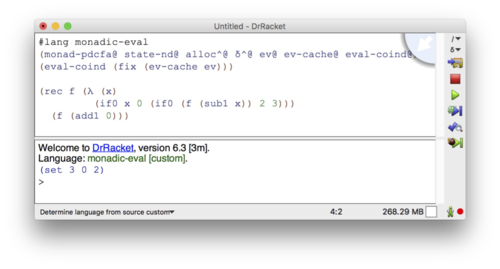
\includegraphics[width=\linewidth]{screen.png}
\caption{Screenshot of Monadic Language}
\label{f:screen}
\end{figure}

\newcommand{\lamif}{«λ⦑IF⦒» }

\section{Formalism}\label{s:formalism}

In this section we formalize our approach to designing static analyzers via
definitional interpreters. The development begins with a ``ground truth''
big-step semantics and concludes with the fixpoint iteration strategy described
in Section~\ref{s:fixing-cache}, which we prove sound w.r.t. a synthesized
abstract semantics. The design is systematic, and applies to arbitrary
programming languages described via big-step operational semantics. We
demonstrate the systematic process as applied to a subset of the language
described in Figure~\ref{f:syntax}, which we call \lamif.

\paragraph{Concrete Semantics}

We begin with the concrete semantics of \lamif as a big-step relation
«ρ,τ⊢e,σ⇓v,σ′», shown in Figures~\ref{f:lamif-syntax}
and~\ref{f:lamif-concrete}. The definition is mostly standard: «ρ» and «σ» are
the environment and store, «e» is the initial expression, and «v» is the
resulting value. The argument «τ» represents ``time'', which when abstracted
supports modeling execution contexts like call-site sensitivity. Concretely
time is modelled as a natural number and represents the number of steps of
execution.

\begin{figure} %{-{
\begin{alignat*}{3}
  n ∈ &&\mathrel{} lits \mathrel{\hphantom{≔}} & \\
  x ∈ &&\mathrel{} vars \mathrel{\hphantom{≔}} & \\
  b ∈ &&\mathrel{}  binop ≔ &\mathrel{} ❴⟬plus⟭, …❵ \\
  e ∈ &&\mathrel{}    exp ⩴ &\mathrel{} n ∣ x ∣ λx.e ∣ e(e) ∣ ⟬if0⟭(e)❴e❵❴e❵ ∣ b(e,e) \\
  ρ ∈ &&\mathrel{}    env ≔ &\mathrel{} var → addr⸤⊥⸥ \\
  σ ∈ &&\mathrel{}  store ≔ &\mathrel{} addr → val⸤⊥⸥ \\
  v ∈ &&\mathrel{}    val ⩴ &\mathrel{} n ∣ ⟨λx.e,ρ⟩ \\
  ℓ ∈ &&\mathrel{}   addr ≔ &\mathrel{} var × time \\
  τ ∈ &&\mathrel{}   time ≔ &\mathrel{} ℕ
\end{alignat*}
\caption{\lamif{} Syntactic Categories}
\label{f:lamif-syntax}
\end{figure} %}-}

\begin{figure} %{-{
\begin{mathpar}

  \inferrule*[left=(Lit)]{ }{ρ , τ ⊢ n , σ ⇓ n , σ}

  \inferrule*[left=(Var)]{ }{ρ , τ ⊢ x , σ ⇓ σ(ρ(x)) , σ}

  \inferrule*[left=(Lam)]{ }{ρ , τ ⊢ λx.e , σ ⇓ ⟨λx.e,ρ⟩ , σ}

  \inferrule*[left=(App),right={\begin{minipage}{2em}\ssmall
    \begin{alignat*}{1}
    \begin{alignedat}{2} 
⟨λx.e′,ρ′⟩ = &\mathrel{} v₁ \\[-0.5em]
        τ′ = &\mathrel{} τ+1 \\[-0.5em]
        ℓ  = &\mathrel{} ⟨x,τ′⟩ \\
      \end{alignedat}
    \end{alignat*}
  \end{minipage}}]{
  ρ       , τ  ⊢ e₁    , σ        ⇓ v₁ , σ₁ \\
  ρ       , τ  ⊢ e₂    , σ₁       ⇓ v₂ , σ₂ \\
  ρ′[x↦ℓ] , τ′ ⊢ e′    , σ₂[ℓ↦v₂] ⇓ v′ , σ₃}
  {ρ      , τ ⊢ e₁(e₂) , σ        ⇓ v′ , σ₃}

  \inferrule*[left=(If-T),right={\ssmall «n=0»}]{
  ρ , τ ⊢ e₁ , σ ⇓ n , σ₁ \\
  ρ , τ ⊢ e₂ , σ₁ ⇓ v , σ₂}
  {ρ , τ ⊢ ⟬if0⟭(e₁)❴e₂❵❴e₃❵ , σ ⇓ v , σ₂}

  \inferrule*[left=(If-F),right={\ssmall «n≠0»}]{
    ρ , τ ⊢ e₁ , σ  ⇓ n , σ₁ \\
    ρ , τ ⊢ e₃ , σ₁ ⇓ v , σ₂}
  {ρ , τ ⊢ ⟬if0⟭(e₁)❴e₂❵❴e₃❵ , σ ⇓ v , σ₂}

  \inferrule*[left=(Bin)]{
  ρ , τ ⊢ e₁ , σ  ⇓ v₁ , σ₁ \\
  ρ , τ ⊢ e₂ , σ₁ ⇓ v₂ , σ₂}
  {ρ , τ ⊢ b(e₁,e₂) , σ ⇓ ⟦b⟧(v₁,v₂) , σ₂}
\end{mathpar}
\caption{\lamif{} Big-step Concrete Semantics}
\label{f:lamif-concrete}
\end{figure} %}-}

\paragraph{Reachability}

The primary limitation of using big-step semantics as a starting point for
abstraction is that intermediate computations are not represented in the model.
For example, consider the program that applies the identity function to an
expression that loops, which we notate «Ω»:
\[ (λx.x)(Ω) \]
A big-step semantics can only describe results of terminating computations, and
because this program never terminates, our big-step semantics relation says
nothing about the behavior of the program. A good static analyzer will explore
the behavior of «Ω» to (possibly) discover that it loops, but more importantly,
to provide analysis results (like data-flow or side-effects) for intermediate
computation states.

The need to analyze intermediate states is the primary reason that big-step
semantics are overlooked as a starting point for abstract interpretation. To
remedy the situation, while remaining in a big-step setting, we introduce a
big-step \emph{reachability semantics}, described by the relation «ρ,τ⊢e,σ⇑ς»
shown in Figure~\ref{f:lamif-reachability}. Configurations «ς» are tuples
«⟨e,ρ,σ,τ⟩», and are reachable when evaluation passes through the configuration
at any point on its way to a final value, or during an infinite loop.

\begin{figure} %{-{
\begin{mathpar}
  \inferrule*[left=(Refl)]{ }{ρ,τ⊢e,σ⇑⟨e,ρ,σ,τ⟩}

  \inferrule*[left=(RApp1)]
   {ρ,τ⊢e₁,σ⇑ς}
   {ρ,τ⊢e₁(e₂),σ⇑ς}

   \inferrule*[left=(RApp2),right={\ssmall «⟨λx.e′,ρ′⟩=v₁»}]
   {  ρ,τ⊢e₁,σ⇓v₁,σ₁
   \\ ρ,τ⊢e₂,σ₁⇑ς}
   {ρ,τ⊢e₁(e₂),σ⇑ς}

   \inferrule*[left=(RApp3),right={\begin{minipage}{2em}\ssmall
       \begin{alignat*}{1}
       \begin{alignedat}{2} 
    ⟨λx.e′,ρ′⟩ = &\mathrel{} v₁ \\[-0.5em]
           τ′ = &\mathrel{} τ+1 \\[-0.5em]
           ℓ  = &\mathrel{} ⟨x,τ′⟩ \\
         \end{alignedat}
       \end{alignat*}
     \end{minipage}}]
  {  ρ,τ⊢e₁,σ ⇓v₁,σ₁
  \\ ρ,τ⊢e₂,σ₁⇓v₂,σ₂
  \\ ρ′[x↦ℓ],τ′⊢e′,σ₂[ℓ↦v₂]⇑ς}
  {ρ,τ⊢e₁(e₂),σ⇑ς}

  \inferrule*[left=(RIf1)]
  {ρ,τ⊢e₁,σ⇑ς}
  {ρ,τ⊢⟬if0⟭(e₁)❴e₂❵❴e₃❵,σ⇑ς}

  \inferrule*[left=(RIf-T),right={\ssmall «n=0»}]
  {  ρ,τ⊢e₁,σ⇓n,σ₁
  \\ ρ,τ⊢e₂,σ₁⇑ς}
  {ρ,τ⊢⟬if0⟭(e₁)❴e₂❵❴e₃❵,σ⇑ς}

  \inferrule*[left=(RIf-F),right={\ssmall «n≠0»}]
  {  ρ,τ⊢e₁,σ⇓n,σ₁
  \\ ρ,τ⊢e₃,σ₁⇑ς}
  {ρ,τ⊢⟬if0⟭(e₁)❴e₂❵❴e₃❵,σ⇑ς}

  \inferrule*[left=(RBin1)]
  {ρ,τ⊢e₁,σ⇑ς}
  {ρ,τ⊢b(e₁,e₂),σ⇑ς}

  \inferrule*[left=(RBin2)]
  {  ρ,τ⊢e₁,σ⇓v₁,σ₁
  \\ ρ,τ⊢e₂,σ₁⇑ς}
  {ρ,τ⊢b(e₁,e₂),σ⇑ς}

\end{mathpar}
\caption{\lamif{} Big-step Reachability Semantics}
\label{f:lamif-reachability}
\end{figure} %}-}

The complete concrete semantics of an expression («e») under environment («ρ»),
store («σ») and time («τ»), which we notate «⟦e⟧⸢bs⸣(ρ,σ,τ)», is then a pairing
of the set of resulting values and final stores («v,σ′»), and the reachable
configurations («ς»):
\begin{alignat*}{1}
  & ⟦e⟧⸢bs⸣(ρ,σ,τ) ≔ \\
  & \hspace{1em}⟨❴⟨v,σ′⟩ ∣ ρ,τ⊢e,σ⇓v,σ′❵,❴ς ∣ ρ,τ⊢e,σ⇑ς❵⟩
\end{alignat*}
We then construct a formal bridge between the complete concrete semantics
(«⟦e⟧⸢bs⸣») and a complete small step semantics, which is traditionally used as
the starting point of abstraction for program analysis:
\begin{alignat*}{1}
  & ⟦e⟧⸢ss⸣(ρ,σ,τ) ≔ \\
  & \hspace{1em}⟨❴⟨v,σ′⟩ ∣ ∀κ. ⟨e,ρ,σ,τ,κ⟩ ↝⸢*⸣ ⟨v,ρ′,σ′,τ′,κ⟩❵ \\
  & \hspace{1em},❴⟨e′,ρ′,σ′,τ′⟩ ∣ ∀κ. ⟨e,ρ,σ,τ,κ⟩ ↝⸢*⸣ ⟨e′,ρ′,σ′,τ′,κ′⧺κ⟩❵⟩
\end{alignat*}
We connect the complete big-step and small-step semantics through the following
theorem:
\begin{theorem}[Complete Big-step/Small-step Equivalence]
  \[ ⟦e⟧⸢bs⸣(ρ,σ,τ) = ⟦e⟧⸢ss⸣(ρ,σ,τ) \]
\end{theorem}
The proof is by induction on the big-step derivation in the «⊆» direction, and
on the transitive small-step derivation in the «⊇» direction.

\paragraph{Collecting Semantics}

Before abstracting the semantics—in pursuit of a sound static analysis
algorithm—we pass through a big-step collecting and reachability semantics,
«ρ,τ⊢e,∿{σ}⇓∿{v},∿{σ}» and «ρ,τ⊢e,∿{σ}⇑∿{ς}», shown in
Figure~\ref{f:lamif-collecting}, where «∿{v}», «∿{σ}» and «∿{ς}» range over
collecting state spaces:
\begin{alignat*}{3}
    ∿{v} ∈ &&\mathrel{} ∿{val}      &\mathrel{} ≔ ℘(val) \\
    ∿{σ} ∈ &&\mathrel{} ∿{store}    &\mathrel{} ≔ addr ↦ ∿{val} \\
    ∿{ς} ∈ &&\mathrel{} ∿{config}   &\mathrel{} ≔ exp × env × ∿{store} × time
\end{alignat*}
The denotation for binary operators («⟦b⟧») is lifted to a collecting
denotation operator «∿{⟦b⟧}»:
\[ ∿{⟦b⟧}(∿{v}₁,∿{v}₂) ≔ ❴⟦b⟧(v₁,v₂) ∣ v₁ ∈ ∿{v}₁ ∧ v₂ ∈ ∿{v}₂❵ \]

\begin{figure*} %{-{
\begin{mathpar}
  \inferrule*[left=(OLit)]{ }{ρ,τ⊢n,∿{σ}⇓❴n❵,∿{σ}}

  \inferrule*[left=(OVar)]{ }{ρ,τ⊢x,∿{σ}⇓∿{σ}(ρ(x)),∿{σ}}

  \inferrule*[left=(OLam)]{ }{ρ,τ⊢λx.e,∿{σ}⇓❴⟨λx.e,ρ⟩❵,∿{σ}}

  \inferrule*[left=(OApp),right={\begin{minipage}{2em}\ssmall
    \begin{alignat*}{1}
    \begin{alignedat}{2} 
              ⟨λx.e′,ρ′⟩ ∈ &\mathrel{} ∿{v}₁ \\[-0.5em]
                      τ′ = &\mathrel{} τ+1 \\[-0.5em]
                      ℓ  = &\mathrel{} ⟨x,τ′⟩
      \end{alignedat}
    \end{alignat*}
  \end{minipage}}]
  {  ρ      ,τ ⊢e₁    ,∿{σ} ⇓∿{v}₁,∿{σ}₁
  \\ ρ      ,τ ⊢e₂    ,∿{σ}₁⇓∿{v}₂,∿{σ}₂
  \\ ρ′[x↦ℓ],τ′⊢e′    ,∿{σ}₂[ℓ↦∿{v}₂]⇓∿{v}′,∿{σ}₃}
  {ρ      ,τ ⊢e₁(e₂),∿{σ} ⇓∿{v}′,∿{σ}₃}

  \inferrule*[left=(OIf-T),right={\ssmall «0∈∿{v}₁»}]
  {  ρ,τ⊢e₁,∿{σ}⇓∿{v}₁,∿{σ}₁
  \\ ρ,τ⊢e₂,∿{σ}₁⇓∿{v},∿{σ}₂}
  {  ρ,τ⊢⟬if0⟭(e₁)❴e₂❵❴e₃❵,∿{σ}⇓∿{v},∿{σ}₂}

  \inferrule*[left=(OIf-F),right={\begin{minipage}{2em}\ssmall
      \begin{alignat*}{2}
        n ∈ &\mathrel{} ∿{v}₁ \\[-0.5em]
        n ≠ &\mathrel{} 0
      \end{alignat*}
    \end{minipage}}]
    {  ρ,τ⊢e₁,∿{σ}⇓∿{v}₁,∿{σ}₁
    \\ ρ,τ⊢e₃,∿{σ}₁⇓∿{v},∿{σ}₂}
    {  ρ,τ⊢⟬if0⟭(e₁)❴e₂❵❴e₃❵,∿{σ}⇓∿{v},∿{σ}₂}

    \inferrule*[left=(OBin)]
  {  ρ,τ⊢e₁,∿{σ}⇓∿{v}₁,∿{σ}₁
  \\ ρ,τ⊢e₂,∿{σ}₁⇓∿{v}₂,∿{σ}₂}
  {  ρ,τ⊢b(e₁,e₂),∿{σ}⇓∿{⟦b⟧}(∿{v}₁,∿{v}₂),∿{σ}₂}

  \inferrule*[left=(ORefl)]{ }{ρ,τ⊢e,∿{σ}⇑⟨e,ρ,∿{σ},τ⟩}

  \inferrule*[left=(ORApp1)]
   {ρ,τ⊢e₁,∿{σ}⇑∿{ς}}
   {ρ,τ⊢e₁(e₂),∿{σ}⇑∿{ς}}

   \inferrule*[left=(ORApp2),right={\ssmall «⟨λx.e′,ρ′⟩∈∿{v}₁»}]
   {  ρ,τ⊢e₁,∿{σ}⇓∿{v}₁,∿{σ}₁
   \\ ρ,τ⊢e₂,∿{σ}₁⇑∿{ς}}
   {ρ,τ⊢e₁(e₂),∿{σ}⇑∿{ς}}

   \inferrule*[left=(ORApp3),right={\begin{minipage}{2em}\ssmall
       \begin{alignat*}{1}
       \begin{alignedat}{2} 
  ⟨λx.e′,ρ′⟩ ∈ &\mathrel{} ∿{v}₁ \\[-0.5em]
           τ′ = &\mathrel{} τ+1 \\[-0.5em]
           ℓ  = &\mathrel{} ⟨x,τ′⟩ \\
         \end{alignedat}
       \end{alignat*}
     \end{minipage}}]
  {  ρ,τ⊢e₁,∿{σ} ⇓∿{v}₁,∿{σ}₁
  \\ ρ,τ⊢e₂,∿{σ}₁⇓∿{v}₂,∿{σ}₂
  \\ ρ′[x↦ℓ],τ′⊢e′,∿{σ}₂[ℓ↦∿{v}₂]⇑∿{ς}}
  {ρ,τ⊢e₁(e₂),∿{σ}⇑∿{ς}}

  \inferrule*[left=(ORIf1)]
  {ρ,τ⊢e₁,∿{σ}⇑∿{ς}}
  {ρ,τ⊢⟬if0⟭(e₁)❴e₂❵❴e₃❵,∿{σ}⇑∿{ς}}

  \inferrule*[left=(ORIf-T),right={\ssmall «0∈∿{v}₁»}]
  {  ρ,τ⊢e₁,∿{σ}⇓∿{v}₁,∿{σ}₁
  \\ ρ,τ⊢e₂,∿{σ}₁⇑∿{ς}}
  {ρ,τ⊢⟬if0⟭(e₁)❴e₂❵❴e₃❵,∿{σ}⇑∿{ς}}

  \inferrule*[left=(ORIf-F),right={\begin{minipage}{2em}\ssmall 
    \begin{alignat*}{2}
      n ∈ &\mathrel{} ∿{v}₁ \\
      n ≠ &\mathrel{} 0
    \end{alignat*}
    \end{minipage}}]
    {  ρ,τ⊢e₁,∿{σ}⇓∿{v}₁,∿{σ}₁
    \\ ρ,τ⊢e₃,∿{σ}₁⇑∿{ς}}
    {ρ,τ⊢⟬if0⟭(e₁)❴e₂❵❴e₃❵,∿{σ}⇑∿{ς}}

  \inferrule*[left=(ORBin1)]
  {ρ,τ⊢e₁,∿{σ}⇑ς}
  {ρ,τ⊢b(e₁,e₂),∿{σ}⇑∿{ς}}

  \inferrule*[left=(ORBin2)]
  {  ρ,τ⊢e₁,∿{σ}⇓∿{v}₁,∿{σ}₁
  \\ ρ,τ⊢e₂,∿{σ}₁⇑∿{ς}}
  {ρ,τ⊢b(e₁,e₂),∿{σ}⇑∿{ς}}

\end{mathpar}
\caption{Big-step Collecting Reachability Semantics}
\label{f:lamif-collecting}
\end{figure*} %}-}

The big-step collecting and reachability relations are structurally similar to
the concrete semantics. The primary differences are using set containment
(«∈») in place of equality («=») when branching on application («⟨λx.e,ρ⟩» in
\textsc{(OApp)}) and conditional («n≟0» in \textsc{(OIf-T)} and
\textsc{(OIf-F)}) expressions.

The big-step collecting reachability semantics is a sound approximation of the
big-step concrete reachability semantics:
\begin{theorem}[Collecting Reachability Semantics Soundness]
  \begin{alignat*}{1}
    & ⦑If:⦒\mathrel{} ρ,τ⊢e,σ⇓v,σ′ \;∧\; η(σ) ⊑ ∿{σ} \\
    & ⦑then:⦒\mathrel{} \mathrel{∃}∿{v},∿{σ}′ \mathrel{⦑s.t.⦒} ρ,τ⊢e,∿{σ}⇓∿{v},∿{σ}′ \;∧\; v ∈ ∿{v} \;∧\; η(σ′) ⊑ ∿{σ}′ \\
    & ⦑and if:⦒\mathrel{} ρ,τ⊢e,σ⇑ς \;∧\; η(σ) ⊑ ∿{σ} \\
    & ⦑then:⦒\mathrel{} \mathrel{∃}∿{ς} \mathrel{⦑s.t.⦒} ρ,τ⊢e,∿{σ}⇑∿{ς} \;∧\; η(ς) ⊑ ∿{ς}
  \end{alignat*}
\end{theorem}
The proof is by induction on the concrete big-step derivation. The extraction
function «η» is defined separately for stores («σ») and configurations («ς»):
\begin{alignat*}{1}
   & η(σ)(ℓ) ≔ ❴σ(ℓ)❵
\\ & η(⟨e,ρ,σ,τ⟩) ≔ ⟨e,ρ,η(σ),τ⟩
\end{alignat*}
and the partial ordering on collecting stores and configurations is pointwise:
\begin{alignat*}{1}
  & ∿{σ}₁ ⊑ ∿{σ}₂ \quad \mathrel{⦑\emph{iff}⦒} \quad ∀ℓ.\mathrel{} ∿{σ}₁(ℓ) ⊆ ∿{σ}₂(ℓ)
  \\ & ⟨e₁,ρ₁,∿{σ}₁,τ₁⟩ ⊑ ⟨e₂,ρ₂,∿{σ}₂,τ₂⟩ \quad \mathrel{⦑\emph{iff}⦒} 
  \\ & \hspace{1em} e₁ = e₂ ∧ ρ₁ = ρ₂ ∧ ∿{σ}₁ ⊑ ∿{σ}₂ ∧ τ₁ = τ₂
\end{alignat*}

\paragraph{Finite Abstraction}

The next step towards a computable static analysis is an abstract semantics
with a finite state space that approximates the big-step collecting semantics,
«♯{ρ},♯{τ}⊢e,♯{σ}⇓♯{v},♯{σ}» and «♯{ρ},♯{τ}⊢e,♯{σ}⇑♯{ς}», shown in
Figure~\ref{f:lamif-abstract}, where «♯{ρ}», «♯{τ}», «♯{v}», «♯{σ}» and «♯{ς}» are finite
abstractions of their collecting counterparts:
\begin{alignat*}{3}
  ♯{ρ} ∈ &&\mathrel{} ♯{env}    &\mathrel{} ≔ var ↦ ♯{addr}⸤⊥⸥ \\
  ♯{ℓ} ∈ &&\mathrel{} ♯{addr}   &\mathrel{} ≔ var × ♯{time} \\
  ♯{τ} ∈ &&\mathrel{} ♯{time}   &\mathrel{} ≔ … \\
  ♯{v} ∈ &&\mathrel{} ♯{val}    &\mathrel{} ≔ … \\
  ♯{σ} ∈ &&\mathrel{} ♯{store}  &\mathrel{} ≔ ♯{addr} ↦ ♯{val} \\
  ♯{ς} ∈ &&\mathrel{} ♯{config} &\mathrel{} ≔ exp × ♯{env} × ♯{store} × ♯{time}
\end{alignat*}
The primary structural difference from the collecting semantics is updating the
store with join («♯{σ}⊔[♯{ℓ}↦♯{v}]») rather than strict replacement
(«∿{σ}[ℓ↦∿{v}]»). This is to preserve soundness in the presence of address
reuse due to the finite size of the address space.

The abstract denotation («♯{⟦b⟧}») is an overapproximation of the collecting
denotation («∿{⟦b⟧}») w.r.t. a Galois connection «∿{val}⇄{α}{γ}♯{val}»:
\[ ♯{⟦b⟧}(♯{v}₁,♯{v}₂) ⊒ α(∿{⟦b⟧}(γ(♯{v}₁),γ(♯{v}₂))) \]
Concretization functions «⌊γ⌋⸤clo⸥», «⌊γ⌋⸤0⸥» and «⌊γ⌋⸤¬0⸥» are computable
finite subsets of the full concretization function «γ» s.t.:
\begin{alignat*}{1}
  & ⌊γ⌋⸤clo⸥(♯{v}) ≔ ❴⟨λx.e,♯{ρ}⟩ ∣ ⟨λx.e,♯{ρ}⟩ ∈ γ(♯{v})❵ \\
  & ⌊γ⌋⸤0⸥(♯{v}) ≔ ❴0 ∣ 0 ∈ γ(♯{v})❵ \\
  & ⌊γ⌋⸤¬0⸥(♯{v}) ≔ ❴¬0 ∣ n ∈ γ(♯{v}) ∧ n≠0❵
\end{alignat*}
Abstract sets «♯{time}» and «♯{val}» are left as parameters to the analysis
along with their operations «♯{next}», «♯{⟦b⟧}», «⌊γ⌋⸤clo⸥», «⌊γ⌋⸤0⸥»,
«⌊γ⌋⸤¬0⸥» and «⊔⸢♯{val}⸣».

The abstract semantics is a sound approximation of the collecting semantics,
which we establish through the theorem:
\begin{theorem}[Abstract Reachability Semantics Soundness]
  \begin{alignat*}{1}
    & ⦑If:⦒\mathrel{} ρ,τ⊢e,∿{σ}⇓∿{v},∿{σ}′ \;∧\; η(ρ) ⊑ ♯{ρ} \;∧\; η(τ) ⊑ ♯{τ} \;∧\; η(∿{σ}) ⊑ ♯{σ} \\
    & ⦑then:⦒\mathrel{} \mathrel{∃}♯{v},♯{σ}′ \mathrel{⦑s.t.⦒} ♯{ρ},♯{τ}⊢e,♯{σ}⇓♯{v},♯{σ}′ \;∧\; η(∿{v}) ⊑ ♯{v} \;∧\; η(∿{σ}′) ⊑ ♯{σ}′ \\
    & ⦑and if:⦒\mathrel{} ρ,τ⊢e,∿{σ}⇑∿{ς} \;∧\; η(ρ) ⊑ ♯{ρ} \;∧\; η(τ) ⊑ ♯{τ} \;∧\; η(∿{σ}) ⊑ ♯{σ} \\
    & ⦑then:⦒\mathrel{} \mathrel{∃}♯{ς} \mathrel{⦑s.t.⦒} ♯{ρ},♯{τ}⊢e,♯{σ}⇑♯{ς} \;∧\; η(∿{ς}) ⊑ ♯{ς}
  \end{alignat*}
\end{theorem}
The proof is by induction on the big-step derivation. The extraction function
«η» is defined separately for environments («ρ»), time («τ»), and collecting
stores («∿{σ}»), values («∿{v}») and configurations («∿{ς}»). «η(τ)» and
«η(∿{v})» are given with parameters «♯{time}» and «♯{val}». «η(ρ)», «η(∿{σ})»
and «η(∿{ς})» are defined pointwise:
\begin{alignat*}{1}
  & η(ρ)(x) ≔ η(ρ(x)) \\
  & η(∿{σ})(♯{ℓ}) ≔ ⨆⸤ℓ ∈ γ(♯{ℓ})⸥η(∿{σ}(ℓ)) \\
  & η(⟨e,ρ,τ,∿{σ}⟩) ≔ ⟨e,η(ρ),η(τ),η(∿{σ})⟩
\end{alignat*}

\begin{figure*} %{-{
\begin{mathpar}
  \inferrule*[left=(ALit)]{ }{♯{ρ},♯{τ}⊢n,♯{σ}⇓♯{η}(n),♯{σ}}

  \inferrule*[left=(AVar)]{ }{♯{ρ},♯{τ}⊢x,♯{σ}⇓♯{σ}(♯{ρ}(x)),♯{σ}}

  \inferrule*[left=(ALam)]{ }{♯{ρ},♯{τ}⊢λx.e,♯{σ}⇓♯{η}(⟨λx.e,♯{ρ}⟩),♯{σ}}

  \inferrule*[left=(AApp),right={\begin{minipage}{2em}\ssmall
    \begin{alignat*}{1}
    \begin{alignedat}{2} 
           ⟨λx.e′,♯{ρ}′⟩ ∈ &\mathrel{} ⌊γ⌋⸤clo⸥(♯{v}₁) \\[-0.5em]
                   ♯{ς}  = &\mathrel{} ⟨e₁(e₂),♯{ρ},♯{σ},♯{τ}⟩ \\[-0.5em]
                   ♯{τ}′ = &\mathrel{} ♯{next}(♯{τ},♯{ς}) \\[-0.5em]
                   ♯{ℓ}  = &\mathrel{} ⟨x,♯{τ}′⟩
      \end{alignedat}
    \end{alignat*}
  \end{minipage}}]
  {  ♯{ρ}      ,♯{τ} ⊢e₁    ,♯{σ} ⇓♯{v}₁,♯{σ}₁
  \\ ♯{ρ}      ,♯{τ} ⊢e₂    ,♯{σ}₁⇓♯{v}₂,♯{σ}₂
  \\ ♯{ρ}′[x↦♯{ℓ}],♯{τ}′⊢e′    ,♯{σ}₂⊔[♯{ℓ}↦♯{v}₂]⇓♯{v}′,♯{σ}₃}
  {♯{ρ}      ,♯{τ} ⊢e₁(e₂),♯{σ} ⇓♯{v}′,♯{σ}₃}

  \inferrule*[left=(AIf-T),right={\ssmall «0∈⌊γ⌋⸤0⸥(♯{v}₁)»}]
  {  ♯{ρ},♯{τ}⊢e₁,♯{σ}⇓♯{v}₁,♯{σ}₁
  \\ ♯{ρ},♯{τ}⊢e₂,♯{σ}₁⇓♯{v},♯{σ}₂}
  {  ♯{ρ},♯{τ}⊢⟬if0⟭(e₁)❴e₂❵❴e₃❵,♯{σ}⇓♯{v},♯{σ}₂}

  \inferrule*[left=(AIf-F),right={\ssmall «¬0∈⌊γ⌋⸤¬0⸥(♯{v}₁)»}]
  {  ♯{ρ},♯{τ}⊢e₁,♯{σ}⇓♯{v}₁,♯{σ}₁
  \\ ♯{ρ},♯{τ}⊢e₃,♯{σ}₁⇓♯{v},♯{σ}₂}
  {  ♯{ρ},♯{τ}⊢⟬if0⟭(e₁)❴e₂❵❴e₃❵,♯{σ}⇓♯{v},♯{σ}₂}

    \inferrule*[left=(ABin)]
    {  ♯{ρ},♯{τ}⊢e₁,♯{σ}⇓♯{v}₁,♯{σ}₁
    \\ ♯{ρ},♯{τ}⊢e₂,♯{σ}₁⇓♯{v}₂,♯{σ}₂}
    {  ♯{ρ},♯{τ}⊢b(e₁,e₂),♯{σ}⇓♯{⟦b⟧}(♯{v}₁,♯{v}₂),♯{σ}₂}

    \inferrule*[left=(ARefl)]{ }{♯{ρ},♯{τ}⊢e,♯{σ}⇑⟨e,♯{ρ},♯{σ},♯{τ}⟩}

  \inferrule*[left=(ARApp1)]
  {♯{ρ},♯{τ}⊢e₁,♯{σ}⇑♯{ς}}
  {♯{ρ},♯{τ}⊢e₁(e₂),♯{σ}⇑♯{ς}}

  \inferrule*[left=(ARApp2),right={\ssmall «⟨λx.e′,♯{ρ}′⟩∈⌊γ⌋⸤clo⸥(♯{v}₁)»}]
  {  ♯{ρ},♯{τ}⊢e₁,♯{σ}⇓♯{v}₁,♯{σ}₁
  \\ ♯{ρ},♯{τ}⊢e₂,♯{σ}₁⇑♯{ς}}
  {♯{ρ},♯{τ}⊢e₁(e₂),♯{σ}⇑♯{ς}}

   \inferrule*[left=(ARApp3),right={\begin{minipage}{2em}\ssmall
       \begin{alignat*}{1}
       \begin{alignedat}{2} 
         ⟨λx.e′,♯{ρ}′⟩ ∈ &\mathrel{} ⌊γ⌋⸤clo⸥(♯{v}₁) \\[-0.5em]
            ♯{ς} = &\mathrel{} ⟨e₁(e₂),♯{ρ},♯{σ},♯{τ}⟩ \\[-0.5em]
           ♯{τ}′ = &\mathrel{} ♯{next}(♯{τ},♯{ς}) \\[-0.5em]
           ♯{ℓ}  = &\mathrel{} ⟨x,♯{τ}′⟩ \\
         \end{alignedat}
       \end{alignat*}
     \end{minipage}}]
     {  ♯{ρ},♯{τ}⊢e₁,♯{σ} ⇓♯{v}₁,♯{σ}₁
       \\ ♯{ρ},♯{τ}⊢e₂,♯{σ}₁⇓♯{v}₂,♯{σ}₂
     \\ ♯{ρ}′[x↦♯{ℓ}],♯{τ}′⊢e′,♯{σ}₂⊔[♯{ℓ}↦♯{v}₂]⇑♯{ς}}
     {♯{ρ},♯{τ}⊢e₁(e₂),♯{σ}⇑♯{ς}}

  \inferrule*[left=(ARIf1)]
  {♯{ρ},♯{τ}⊢e₁,♯{σ}⇑♯{ς}}
  {♯{ρ},♯{τ}⊢⟬if0⟭(e₁)❴e₂❵❴e₃❵,♯{σ}⇑♯{ς}}

  \inferrule*[left=(ARIf-T),right={\ssmall «0∈⌊γ⌋⸤0⸥(♯{v}₁)»}]
  {  ♯{ρ},♯{τ}⊢e₁,♯{σ}⇓♯{v}₁,♯{σ}₁
  \\ ♯{ρ},♯{τ}⊢e₂,♯{σ}₁⇑♯{ς}}
  {♯{ρ},♯{τ}⊢⟬if0⟭(e₁)❴e₂❵❴e₃❵,♯{σ}⇑♯{ς}}

  \inferrule*[left=(ARIf-F),right={\ssmall «¬0∈⌊γ⌋⸤¬0⸥(♯{v}₁)»}]
    {  ♯{ρ},♯{τ}⊢e₁,♯{σ}⇓♯{v}₁,♯{σ}₁
    \\ ♯{ρ},♯{τ}⊢e₃,♯{σ}₁⇑♯{ς}}
    {♯{ρ},♯{τ}⊢⟬if0⟭(e₁)❴e₂❵❴e₃❵,♯{σ}⇑♯{ς}}

  \inferrule*[left=(ARBin1)]
  {♯{ρ},♯{τ}⊢e₁,♯{σ}⇑ς}
  {♯{ρ},♯{τ}⊢b(e₁,e₂),♯{σ}⇑♯{ς}}

  \inferrule*[left=(ARBin2)]
  {  ♯{ρ},♯{τ}⊢e₁,♯{σ}⇓♯{v}₁,♯{σ}₁
  \\ ♯{ρ},♯{τ}⊢e₂,♯{σ}₁⇑♯{ς}}
  {♯{ρ},♯{τ}⊢b(e₁,e₂),♯{σ}⇑♯{ς}}

\end{mathpar}
\caption{Big-step Abstract Reachability Semantics}
\label{f:lamif-abstract}
\end{figure*} %}-}

\paragraph{Computing the Analysis}

An analysis for the program «e₀» w.r.t. the abstract semantics is some cache
«\$ ∈ ♯{config} ↦ ℘(♯{val} × ♯{store})» that maps all configurations reachable
from the initial configuration «⟨e₀,♯{ρ}₀,♯{σ}₀,♯{τ}₀⟩» to their final values
and stores «♯{v},♯{σ}», which we notate «\$ ⊨ e₀»:
\begin{alignat*}{2}
  \$ ⊨ e₀ \quad\quad \mathrel{⦑\emph{iff}⦒} \quad\quad & 
    \begin{alignedat}{2}
    %⦑\emph{forall}⦒ & \mathrel{} e,♯{ρ},♯{σ},♯{τ},♯{v},♯{σ}′: \\
    ⦑\emph{If:}⦒     & \mathrel{} ♯{ρ}₀,♯{τ}₀⊢e₀,♯{σ₀}⇑⟨e,♯{ρ},♯{σ},♯{τ}⟩ \\
    ⦑\emph{and:}⦒    & \mathrel{} ♯{ρ},♯{τ}⊢e,♯{σ}⇓♯{v},♯{σ}′  \\ 
    ⦑\emph{then:}⦒   & \mathrel{} ⟨♯{v},♯{σ}′⟩ ∈ \$(⟨e,♯{ρ},♯{σ},♯{τ}⟩)
      \end{alignedat}
\end{alignat*}
The best cache «\$⁺» is then computed as the least fixed point of the
functional «ℱ»:
\begin{alignat*}{1}
  & ℱ ∈ (♯{config} ↦ ℘(♯{val}×♯{store})) → (♯{config} ↦ ℘(♯{val}×♯{store})) \\
  & ℱ ≔ λ\$.  \\
  &  \hspace{1em} ⨆⸤⟨e,♯{ρ},♯{σ},♯{τ}⟩∈\$⸥ \begin{cases}
     ❴ ⟨e,♯{ρ},♯{σ},♯{τ}⟩ ↦ ❴⟨♯{v},♯{σ}′⟩❵ ∣ ♯{ρ},♯{τ}⊢e,♯{σ}⇓⸢\$⸣♯{v},♯{σ}′ ❵ \\
     ❴ ♯{ς} ↦ ❴❵ ∣ ♯{ρ},♯{τ}⊢e,♯{σ}⇑⸢\$⸣♯{ς}❵
   \end{cases} \\
\end{alignat*}
and defined:
\[ \$⁺ ≔ ⦑\emph{lfp}⦒ (λ\$.\mathrel{} ℱ(\$)  ⊔ ❴⟨e₀,♯{ρ}₀,♯{σ}₀,♯{τ}₀⟩ ↦ ❴❵❵) \]
The relations «♯{ρ},♯{τ}⊢e,♯{σ}⇓⸢\$⸣♯{v},♯{σ}′» and «♯{ρ},♯{τ}⊢e,♯{σ}⇑⸢\$⸣♯{ς}»
are modified versions of the original abstract semantics, but with recursive
judgements replaced by «⟨♯{v},♯{σ}′⟩ ∈ \$(e,♯{ρ},♯{σ},♯{τ})» and «♯{ς} ∈
\$(e,♯{ρ},♯{σ},♯{τ})» respectively. Therefore «ℱ» is not recursive; the
recursion in the relations is lifted to the outer fixpoint of the analysis.
Because the state space «♯{config} ↦ ℘(♯{val}×♯{store})» is finite and «ℱ» is
monotonic, «\$⁺» can be computed algorithmically in finite time by a simple
Kleene fixed-point iteration. See Nielson et al~\cite{dvanhorn:Neilson:1999}
for more background and examples of static analyzers computed in this style,
and from which the current development was largely inspired.
\begin{theorem}[Algorithm Correctness]
  «\$⁺» is a valid analysis for «e₀», that is:
  \[ \$⁺ ⊨ e₀ \]
\end{theorem}
The proof is by induction on the assumed derivations
«♯{ρ}₀,♯{τ}₀⊢e₀,♯{σ}₀⇑⟨♯{e},♯{ρ},♯{σ},♯{τ}⟩» and «♯{ρ},♯{τ}⊢e,♯{σ}⇓♯{v},♯{σ}′»,
and utilizes the fact that «\$⁺» is a fixed point, that is:
\[ ℱ(\$⁺) = \$⁺ \]
Our final theorem relates the analysis cache «\$⁺» back to the concrete
semantics of the initial program as a sound approximation:
\begin{theorem}[Algorithm Soundness]
  \begin{alignat*}{1}
    & ⦑If:⦒ \mathrel{} ρ₀,τ₀⊢e₀,σ₀⇑⟨e,ρ,σ,τ⟩ \;∧\; ρ,τ⊢e,σ⇓v,σ′  \\
    & ⦑then:⦒ \mathrel{} ∃♯{ρ},♯{τ},♯{σ},♯{v},♯{σ}′ \mathrel{⦑s.t.⦒}  ⟨♯{v},♯{σ}′⟩ ∈ \$⁺(⟨e,♯{ρ},♯{σ},♯{τ}⟩)  \\
    & \hspace{1em} ∧\; η(ρ) ⊑ ♯{ρ} \;∧\; η(τ) ⊑ ♯{τ} \;∧\; η(σ) ⊑ ♯{σ} \\
    & \hspace{1em} ∧\; η(v) ⊑ ♯{v} \;∧\; η(σ′) ⊑ ♯{σ}′
  \end{alignat*}
\end{theorem}
The proof follows by composing Theorems~1-4.

\paragraph{Computing with Definitional Interpreters}

The algorithm described in Section~\ref{s:fixing-cache} is a more efficient strategy for
computing «\$⁺» using an extensible open-recursive definitional interpreter.
This technique is general, and bridges the gap between the big-step abstract
semantics formalized in this section and the definitional interpreters we wish
to execute to obtain analyses.

An extensible open-recursive definitional interpreter for \lamif (the small
language formalized in this section) has domain:
\begin{alignat*}{1}
  & ℰ ∈ Σ → Σ \quad ⦑\emph{where}⦒ \quad Σ ≔ ♯{config} → ℘(♯{val}×♯{store})
\end{alignat*}
and is defined such that its denotational-fixpoint («Y(ℰ)») recovers concrete
interpretation when instantiated with the concrete state-space. For example,
the recursive case for binary operator expressions is defined:
\begin{alignat*}{1}
  & ℰ(ℰ′)(⟨b(e₁,e₂),♯{ρ},♯{σ},♯{τ}) ≔  \\
  & \hspace{1em} ❴\mathrel{} ♯{⟦b⟧}(♯{v}₁,♯{v₂}) \\
  & \hspace{1em} ∣\mathrel{} ⟨♯{v}₁,♯{σ}₁⟩ ∈ ℰ′(⟨e₁,♯{ρ},♯{σ},♯{τ}⟩) ∧ ⟨♯{v}₂,♯{σ}₂⟩ ∈ ℰ′(⟨e₂,♯{ρ},♯{σ}₁,♯{τ}⟩) ❵
\end{alignat*}
The iteration strategy to analyze the program «e₀» is then to run «e₀» using
«ℰ», but intercepting recursive calls to:
\begin{enumerate}
  \item cache results for all intermediate configurations «♯{ς}», and
  \item cache seen states to prevent infinite loops.
\end{enumerate}
(1) is required to fulfill the specification that «\$⁺» include results for all
reachable configurations from «e₀», and (2) is required to reach a fixed point
of the analysis. To track this extra information we add functional state to the
interpreter (which was done through a monad transformer in the tutorial
development) of type:
\[ ♯{cache} ≔ ♯{config} ↦ ℘(♯{val}×♯{store}) \]
such that the open-recursive evaluator has type:
\begin{alignat*}{1}
  & ℰ ∈ Σ → Σ \quad ⦑\emph{where}⦒ \\
  & \hspace{1em} Σ ≔ ♯{config}×♯{cache} → ℘(♯{val}×♯{store})×♯{cache}
\end{alignat*}
The iteration to compute «\$⁺» given «ℰ» is then defined:
\begin{alignat*}{1}
  & \hspace{0em} \$⁺ ≔ ⦑\emph{lfp}⦒(λ\$ᵒ. \\
  & \hspace{1em} \mathrel{⟬let⟭} ℰ⋆ ≔ Y(λℰ′. \\
  & \hspace{2em}    ℰ(λ⟨♯{ς},\$ⁱ⟩. \\
  & \hspace{3em}      \mathrel{⟬if⟭} ♯{ς} ∈ \$ⁱ \mathrel{⟬then⟭} ⟨\$ⁱ(♯{ς}),\$ⁱ⟩ \mathrel{⟬else⟭} \\
  & \hspace{3em}      \mathrel{⟬let⟭} ⟨♯{VS},\$⸢i\prime⸣⟩ ≔ ℰ′(♯{ς},\$ⁱ[♯{ς}↦\$ᵒ(♯{ς})]) \\
  & \hspace{3em}      \mathrel{⟬in⟭} ⟨♯{VS},\$⸢i\prime⸣[♯{ς}↦♯{VS}]⟩)) \\
  & \hspace{1em} \mathrel{⟬in⟭} π₂(ℰ⋆(⟨e₀,♯{ρ}₀,♯{σ}₀,♯{τ}₀⟩,❴❵)))
\end{alignat*}
The fixed interpreter «ℰ⋆» calls the unfixed interpreter «ℰ», but intercepts
recursive calls to perform (1) and (2) described above. When loops are
detected, the results from the previous complete result «\$ᵒ» is used, and the
outer fixpoint of the algorithm computes the least fixed point of this «\$ᵒ».

The end result is that, rather than compute analysis results and reachable
states naively with Kleene fixpoint iteration, we are able to reuse the
standard definitional interpreter—written in open-recursive form—to
simultaneously explore reachable states, cache intermediate configurations, and
iterate towards a least fixpoint solution for the analysis. This method is more
efficient, and reuses an extensible definitional interpreter which can recover
a wide range of analyses, including concrete interpretation.

\paragraph{Widening}

Two forms of widening can be employed to the semantics and iteration algorithm
to achieve acceptable performance for the abstract interpreter.

The first form of widening is to widen the store in the result set
«℘(♯{val}×♯{store})» to «℘(♯{val})×♯{store}» in the evaluator «ℰ»:
\begin{alignat*}{1}
  & ℰ ∈ Σ → Σ \quad ⦑\emph{where}⦒ \\
  & \hspace{1em} Σ ≔ ♯{config} × ♯{cache} → ℘(♯{val})×♯{store}×♯{cache}
\end{alignat*}
We perform this widening systematically and with no added effort through the
use of Galois Transformers in Section~\ref{s:widening}. The iteration strategy for
this widened state space is the same as before, which computes a fixed point of
the outer cache «\$ᵒ».

The next form of widening is to pull the store out of the configuration space
\emph{entirely}, that is:
\begin{alignat*}{2}
  ♯{ς} ∈ &\mathrel{} ♯{config} ≔ exp × ♯{env} × ♯{time} \\
    \$ ∈ &\mathrel{} ♯{cache} ≔ ♯{config} ↦ ℘(♯{val})
\end{alignat*}
and:
\begin{alignat*}{1}
  & ℰ ∈ Σ → Σ \quad ⦑\emph{where}⦒ \\
  & \hspace{1em} Σ ≔ ♯{config}×♯{store}×♯{cache} → ℘(♯{val})×♯{store}×♯{cache}
\end{alignat*}
The fixed point iteration then finds a mutual least fixed-point of both the
outer cache «\$ᵒ» \emph{and} the store «♯{σ}»:
\begin{alignat*}{1}
  & \hspace{0em} ⟨\$⁺,♯{σ}⁺⟩ ≔ ⦑\emph{lfp}⦒(λ⟨\$ᵒ,♯{σ}⟩. \\
  & \hspace{1em} \mathrel{⟬let⟭} ℰ⋆ ≔ Y(λℰ′. \\
  & \hspace{2em}    ℰ(λ⟨♯{ς},♯{σ}ⁱ,\$ⁱ⟩. \\
  & \hspace{3em}      \mathrel{⟬if⟭} ♯{ς} ∈ \$ⁱ \mathrel{⟬then⟭} ⟨\$ⁱ(♯{ς}),σⁱ,\$ⁱ⟩ \mathrel{⟬else⟭} \\
  & \hspace{3em}      \mathrel{⟬let⟭} ⟨♯{V},♯{σ}⸢i\prime⸣,\$⸢i\prime⸣⟩ ≔ ℰ′(♯{ς},♯{σ}ⁱ,\$ⁱ[♯{ς}↦\$ᵒ(♯{ς})]) \\
  & \hspace{3em}      \mathrel{⟬in⟭} ⟨♯{V},♯{σ}⸢i\prime⸣,\$⸢i\prime⸣[♯{ς}↦♯{V}]⟩)) \\
  & \hspace{1em} \mathrel{⟬in⟭} π⸤2×3⸥(ℰ⋆(⟨e₀,♯{ρ}₀,♯{τ}₀⟩,♯{σ},❴❵)))
\end{alignat*}
This second version of widening, which computes a fixpoint also over the store,
recovers a so-called \emph{flow-insensitive} analysis. In this model, all
program states are re-analyzed in the store resulting from execution. Also, the
cache («\$») does not index over store states «♯{σ}» in its domain, greatly
reducing its size, and leading to a much more efficient (although less precise)
static analyzer.

\paragraph{Recovering Classical 0CFA}

From the fully widened static analyzer, which computes a mutual fixpoint
between a cache and store, we can easily recover a classical 0CFA analysis. We
do this by instantiating «♯{time}» to the singleton abstraction «❴•❵», as was
shown in the original work on AAM~\cite{dvanhorn:VanHorn2010Abstracting}. In
this setting, the lexical environment «ρ» is uniquely determined by the program
expression «e», and can therefore be eliminated, resulting in the analysis
state space:
\begin{alignat*}{2}
  ♯{ς} ∈ &\mathrel{} ♯{config} ≔ exp \\
    \$ ∈ &\mathrel{} ♯{cache} ≔ exp ↦ ℘(♯{val}) \\
  ♯{σ} ∈ &\mathrel{} ♯{store} ≔ var ↦ ℘(♯{val})
\end{alignat*}
The specification for the analysis and the fully store-widened least
fixed-point iteration for computing it recovers the constraint-based
description of 0CFA given by Nielson \emph{et al}
in~\cite{dvanhorn:Neilson:1999}, where 0CFA is defined as the smallest cache
(«\$») and store («σ») which satisfy a co-inductively defined judgment:
\[ \$,σ ⊨ e \]

\paragraph{Recovering Pushdown Analysis}

We borrow from the recent result in pushdown analysis~\cite{local:p4f} which shows
that full pushdown precision can be achieved in a small-step store-widened
abstract semantics by allocating continuations using the address space of
program expressions paired with abstract environments («⟨e,♯{ρ}⟩»). In other
words, «⟨e,♯{ρ}⟩» is sufficient to achieve full pushdown precision because
the tuple uniquely identifies the evaluation context up to the final result of
evaluation.

Our fully widened semantics recovers this pushdown setting because the
cache maps tuples «⟨e,♯{ρ},♯{τ}⟩», which trivially contains «⟨e,♯{ρ}⟩».
Furthermore, we can immediately see that the abstract time component «♯{τ}» is
redundant, and can eliminate it from the cache, resulting in analysis state
space:
\begin{alignat*}{2}
  ♯{ς} ∈ &\mathrel{} ♯{config} ≔ exp × ♯{env} × ♯{time} \\
    \$ ∈ &\mathrel{} ♯{cache} ≔ exp × ♯{env} ↦ ℘(♯{val}) \\
  ♯{σ} ∈ &\mathrel{} ♯{store} ≔ var × ♯{addr} ↦ ℘(♯{val})
\end{alignat*}

An advantage of our setting is that we recover pushdown analysis also for
varying degrees of store-widening, which is not the case in Gilray \emph{et
al}~\cite{local:p4f}, although pushdown precision for non-widened semantics has been
shown before in Johnson and Van Horn~\cite{dvanhorn:Johnson2014Abstracting}.
Furthermore, the implementation of our analyzer achieves this precision by
precise call-return matching in the defining metalanguage of a definitional
interpreter, requiring no added instrumentation to the state-space of the
analyzer (although in the case of Gilray \emph{et al} the instrumentation is
minor).

Going back to Nielson et al~\cite{dvanhorn:Neilson:1999}, it would be interesting to redevelop
their constraint-based analysis descriptions of kCFA in a form that
recovers pushdown precision. Such an exercise would amount to translating our
big-step abstract semantics instantiated to kCFA to a constraint system. The
resulting system would differ from classical kCFA by the addition of
environments «♯{ρ}» (which Nielson et al call context environments) to the
domain of the cache. In this way our formal framework is able to bridge the gap
between results in pushdown analysis described via small-step machines \emph{a
la} Van Horn and Might~\cite{dvanhorn:VanHorn2010Abstracting}, and
constraint-based systems \emph{a la} Nielson et al for which pushdown analysis
has yet to be described effectively.

\section{Related Work}

This work draws upon and re-presents many existing ideas from the literature on
abstract interpretation for higher-order languages.  In particular, it closely
follows the abstracting abstract
machine~\cite{dvanhorn:VanHorn2010Abstracting,dvanhorn:VanHorn2012Systematic}
approach to deriving abstract interpreters from semantics for higher-order
languages.  The key difference here is that we have done it in the setting of a
monadic definitional interpreter instead of an abstract machine.  This involved
a novel caching mechanism and fixed-point algorithm, but otherwise followed the
same recipe.  Remarkably, the pushdown property is simply inherited from the
meta-language rather than require explicit mechanisms within the abstract
interpreter.

The use of monads and monad transformers to make extensible (concrete)
interpreters is a well-known
idea~\cite{davdar:Moggi:1989:Monads,local:steele-popl94,dvanhorn:Liang1995Monad},
which we have extended to work for compositional abstract interpreters.  The
use of monads and monad transformers in machine based-formulatons of abstract
interpreters has previously been explored by Sergey, \emph{et
al.}~\cite{dvanhorn:Sergey2013Monadic} and Darais \emph{et
al.}~\cite{local:darais-oopsla2015}, respectively.  Darais has also shown that
certain monad transformers are also \emph{Galois transformers}, i.e. they
compose to form monads that are Galois connections.  This idea may pave a path
forward for having both componential code \emph{and proofs} for abstract
interpreters in the style presented here.

The caching mechanism used to ensure termination in our abstract interpreter is
similar to that used by Johnson and Van
Horn~\cite{dvanhorn:Johnson2014Abstracting}.  They use a local- and
meta-memoization table in a machine-based interpreter to ensure termination for
a pushdown abstract interpreter.  This mechanism is in turn reminiscent of
Glück's use of memoization in an interpreter for two-way non-deterministic
pushdown automata~\cite{local:gluck-schmidtfest13}.

Vardoulakis, who was the first to develop the idea of a pushdown abstraction
for higher-order flow analysis~\cite{dvanhorn:Vardoulakis2011CFA2}, formalized
CFA2 using a CPS model, which is similar in spirit to a machine-based model.
However, in his dissertation~\cite{local:vardoulakis-diss12} he sketches an
alternative presentation dubbed ``Big CFA2'' which is a big-step operational
semantics for doing pushdown analysis quite similar in spirit to the approach
presented here.  One key difference is that Big CFA2 fixes a particular coarse
abstraction of base values and closures---for example, both branches of a
conditional are always evaluated.  Consequently, it only uses a single
iteration of the abstract evaluation function, similar to the \emph{unsound}
approach of Section~\ref{s:cache} and avoids the need for the cache-based
fixed-point of Section~\ref{s:fixing-cache}.  We don't believe Big CFA2 as
stated is unsound, however if the underlying abstractions were tightened, it
appears it would run in to the same issues identified here.

Our formulation of a pushdown abstract interpreter computes an abstraction
similar to the many existing variants of pushdown flow analysis~\cite%
{dvanhorn:Vardoulakis2011CFA2%
,dvanhorn:Earl2010Pushdown%
,local:vardoulakis-diss12%
,dvanhorn:VanHorn2012Systematic%
,dvanhorn:Earl2012Introspective%
,dvanhorn:Johnson2014Abstracting%
,dvanhorn:Johnson2014Pushdown%
,local:p4f%
}.
% @;{ Our incorporation of an
% abstract garbage collector into a pushdown abstract interpreter
% achieves a similar goal as that of so-called @emph{introspective}
% pushdown abstract interpreters@~cite[earl-icfp12 johnson-jfp14].  }
The mixing of symbolic execution and abstract intrepretation is similar in
spirit to the \emph{logic flow analysis} of Might~\cite{local:might-popl07},
albeit in a pushdown setting and with a stronger notion of negation; generally,
our presentation resembles traditional formulations of symbolic execution more
closely.  Our approach to symbolic execution only handles the first-order case
of symbolic values, as is traditional.  However, Nguyễn's work on higher-order
symbolic execution~\cite{dvanhorn:Nguyen2015Relatively} demonstrates how to
scale to behavioral symbolic values.  In principle, it should be possible to
handle this case in our approach by adapting Nguyễn's method to a formulation
in a compositional evaluator.

We have eschewed soundness proofs in this paper.  This is done in part to
emphasize the pearly intuitions and constructions of abstract definitional
interpreters and in part because it is far less clear how to prove soundness
when compared to the machine-based formulations. Part of the difficulty stems
from the set-up to support extensibility. As mentioned previously, perhaps
Galois transformers~\cite{local:darais-oopsla2015} can help with this aspect.
But even if we fixed a particular set of components and monad transformer
stack, we run up against the challenge of having to prove soundness in the
presence of concrete computations which may not terminate. Handling this in the
small-step setting is easy using a preservation argument, but it's not clear
how to do it with our approach.  Rompf and Amin's recent work on proving type
soundness with definitional interpreters~\cite{local:rompf-arxiv2015} appears
revelant and perhaps paves a way forward.

Now that we have abstract interpreters formulated with a basis in abstract
machines and with a basis in monadic interpreters, an obvious question is can
we obtain a correspondence between them similar to the functional
correspondence between their concrete
counterparts~\cite{dvanhorn:Ager2005Functional}.  An interesting direction for
future work is to try to apply the usual tools of defunctionalization, CPS, and
refocusing to see if we can interderive these abstract semantic artifacts.

\section{Conclusions}

We have shown that a definitional interpreter written in monadic style
can express a wide variety of semantics, such as the usual concrete
semantics, collecting semantics, abstract interpretations, symbolic
execution, and several combinations thereof. 

Remarkably, we observe that our abstract interpreter implements a form
of pushdown abstraction in which calls and returns are always properly
matched in the abstract semantics.  True to the definitional style of
Reynolds, the evaluator involves no explicit mechanics to achieve this
property; it is simply inherited from the defining language.

We believe this formulation of higher-order abstract interpretation
offers a promising new foundation for making re-usable components for
the static analysis and verification of higher-order programs.


%\appendix
%\section{Appendix Title}

%\acks
% We thank Sam Tobin-Hochstadt and Dionna Glaze for several fruitful
% conversations while developing the ideas in this work.

\balance
\bibliographystyle{abbrvnat}
\bibliography{davdar,dvanhorn,local}

\end{document}

%\lstset
% {language=Lisp
% ,extendedchars=true
% ,inputencoding=utf8
% ,mathescape=true
% ,escapechar=`
% ,upquote=true
% ,basicstyle=\ttfamily\color{ParenColor}
% ,commentstyle=\color{CommentColor}
% ,alsoletter=+-*/?'\#0123456789^
% ,identifierstyle=\color{IdentifierColor}
% ,emph=%
%  {return,bind
%  ,zero?
%  ,ask-env,local-env
%  ,ext,find,alloc
%  ,get-store,put-store,update-store
%  ,tell
%  ,get-dead,put-dead,update-dead
%  ,fail,mplus
%  ,get-,put-,update-
%  ,ask-,local-
%  }
% ,emphstyle=\color{IdentifierColor}\emph
% ,classoffset=1
% ,keywords={'add1,'sub1,'+,'-,'*,'quotient,'failure,'N,\#t,\#f,0,1,2,3,4,5,6,7,8,9}
% ,keywordstyle=\color{ValueColor}
% }

